\documentclass[12pt, a4paper]{AnantDocumentation}

\title{EEE F435: Digital Image Processing \\ Assignment 3}
\author{Pranav Chandra N. V. \\ 2023AAPS0013P}
\date{28th November, 2025}

\backgroundsetup{
	contents = ""
}

\usepackage[T1]{fontenc}
\usepackage{listings}
\lstset{
	backgroundcolor=\color{white},
	basicstyle=\ttfamily\small,
	breaklines=true,
	frame=single,
	numbers=left,
	numberstyle=\tiny,
	keywordstyle=\color{blue},
	commentstyle=\color{gray},
	stringstyle=\color{red},
	showstringspaces=false
}

\begin{document}
\maketitle
\tableofcontents
\listoffigures

\section{Introduction}
\label{sec:introduction}
This assignment had the goal of looking into the implementation of various compression algorithms, both for text, greyscale images, and binary images.
The assignment comprised of two distinct questions, the first being focused on text compression using LZ77, LZ78 and LZW encoding styles, and the second being focused on image compression using Predictive Coding, Block Transforms and Wavelet Encoding.

Images from both the first and second assignment were used for the second part of this assignment. The originals are shown below for reference in Figure \ref{fig:original-images}.

\begin{figure}[h!]
	\centering
	\begin{subfigure}{0.45\textwidth}
		\centering
		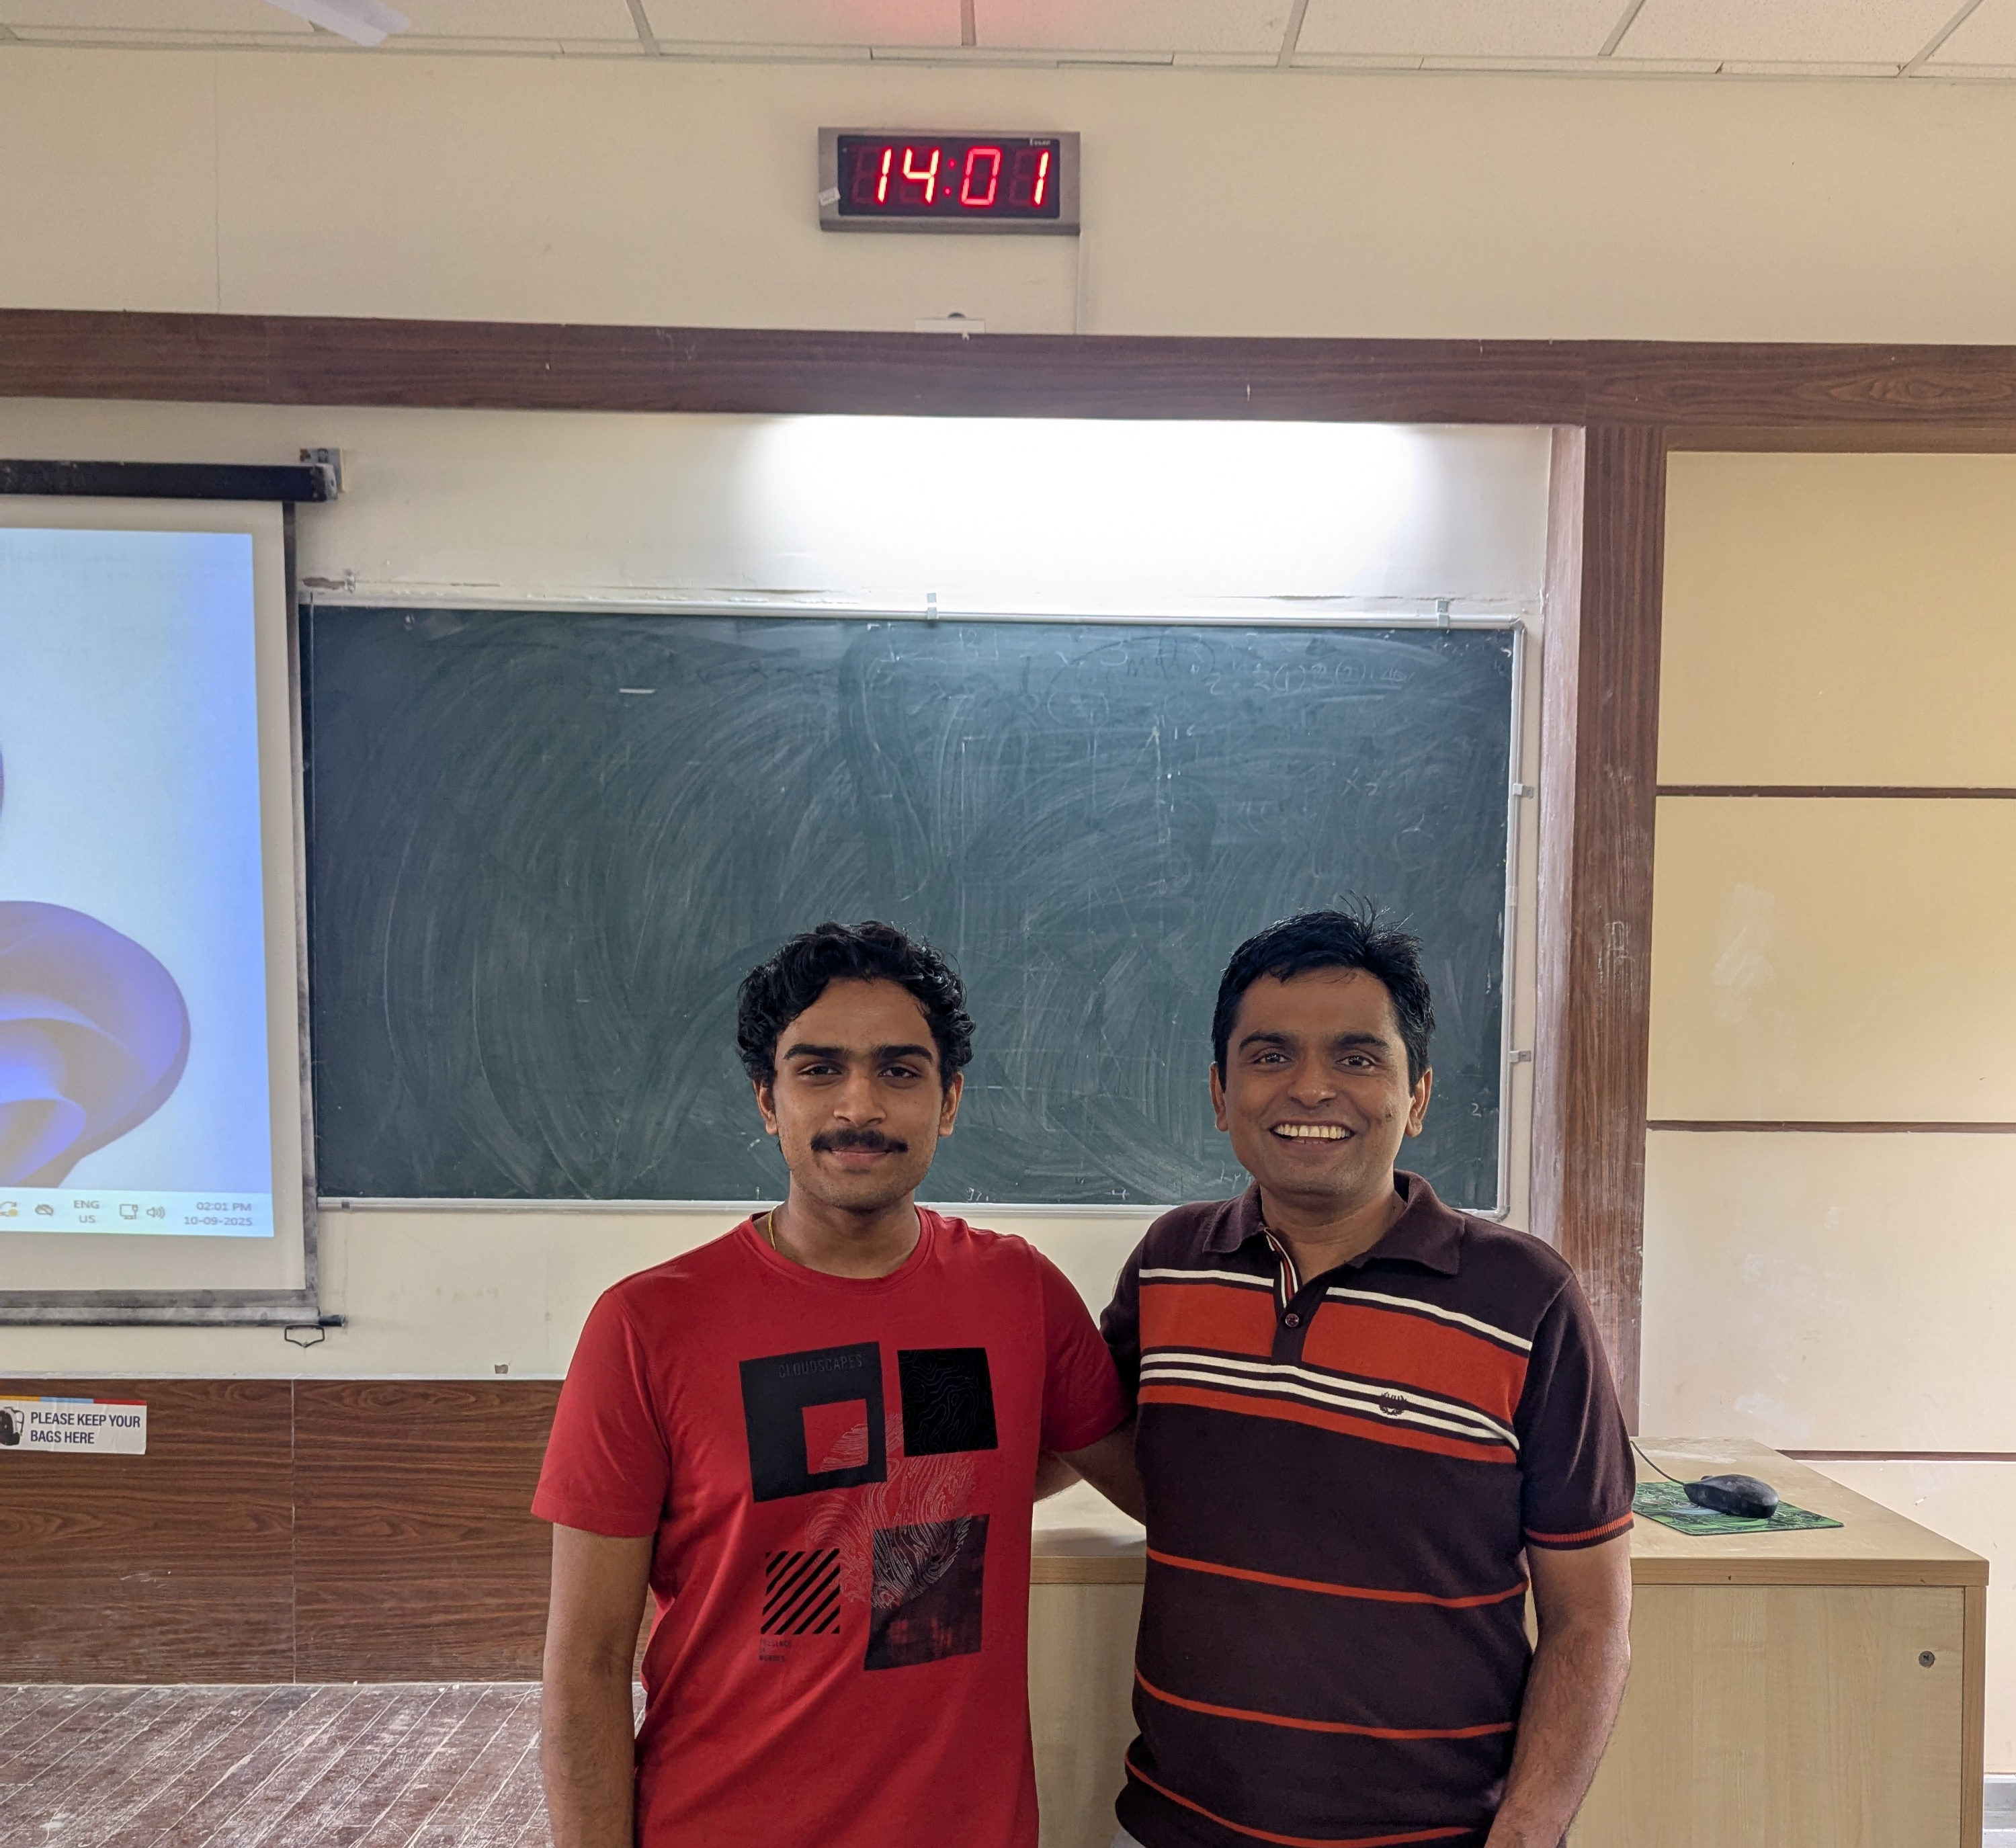
\includegraphics[width=0.7\textwidth]{images/assignment1-image.png}
		\caption{Assignment 1 Image}
		\label{fig:assignment-1-og}
	\end{subfigure}
	\hfill
	\begin{subfigure}{0.45\textwidth}
		\centering
		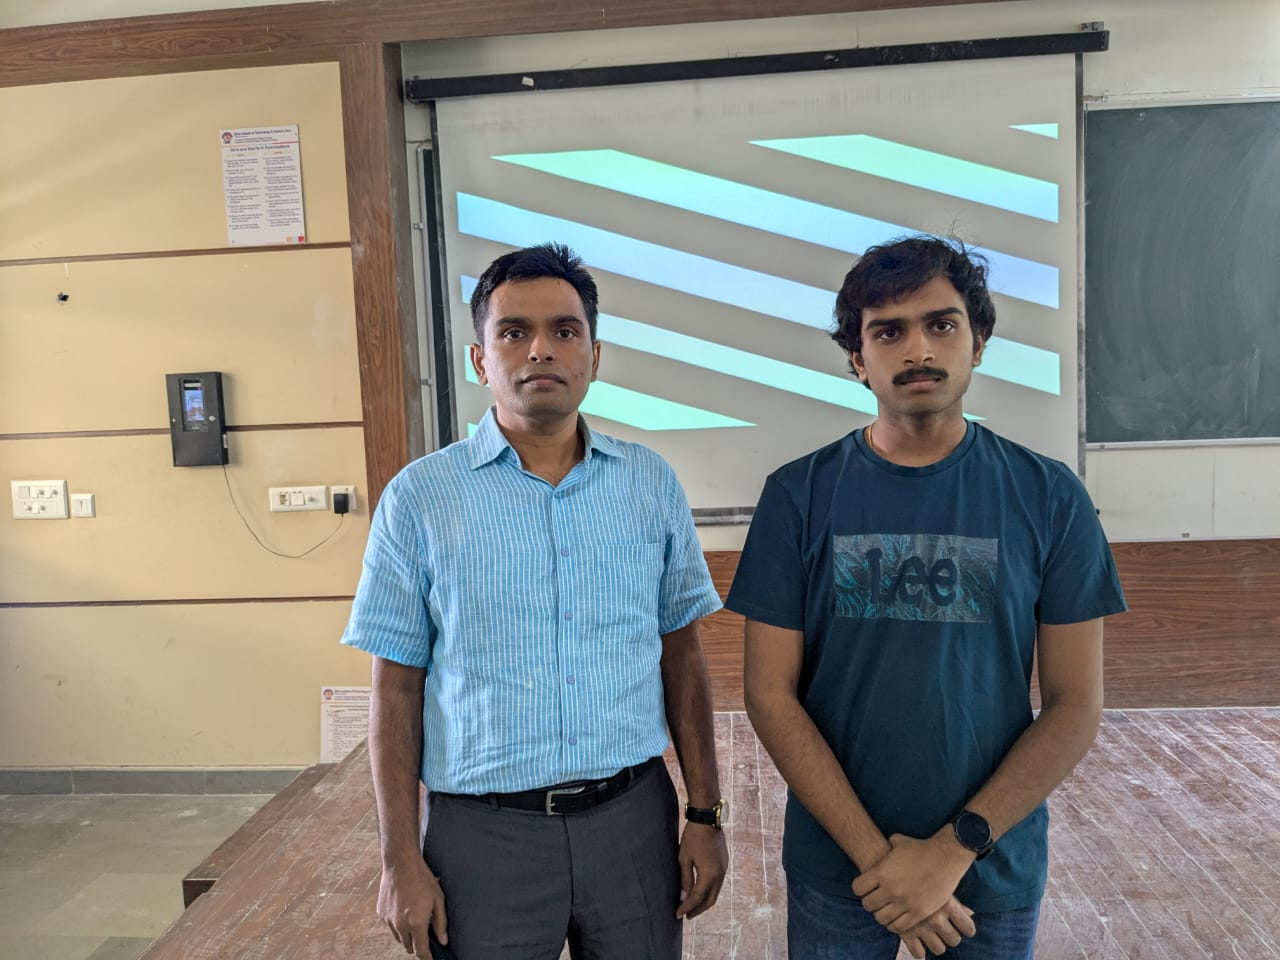
\includegraphics[width=0.85\textwidth]{images/assignment2-image.png}
		\caption{Assignment 2 Image}
		\label{fig:assignment-2-og}
	\end{subfigure}
	\caption{Original Images From Prior Assignments}
	\label{fig:original-images}
\end{figure}

\newpage
\section{Text Compression}
\label{sec:text-compression}
The first part of the assignment involved implementing three different text compression algorithms, namely LZ77, LZ78 and LZW. The primary string used was \textbf{INKYPINKYPONKY} as defined in the assignment brief.

The only issue with the given text, was the short length. This length made it difficult to demonstrate the effectiveness of the algorithms, as the overhead of storing pointers and dictionaries often outweighed the benefits of compression. 
As such, an extension was made, using the string:
\begin{center}
	\textbf{INKYPINKYPONKYPONKYPINKYINKYNKYPONKY}
\end{center}
which is a repetition of the original string with some additional characters to increase length and redundancy.

\subsection{LZ77 Compression}
\label{subsec:lz77}
LZ77 compression works by replacing repeated occurrences of data with references to a single copy existing earlier in the uncompressed data stream. The algorithm uses a sliding window approach, where a search buffer (containing previously seen data) and a look-ahead buffer (containing upcoming data) are maintained.

\subsubsection{Basic Implementation}
\label{subsubsec:lz77-basic}
For this implementation, a window size of 10 characters, with a 6-length search buffer and a 4-length look-ahead buffer was used. The compressed output is represented as tuples of the form (offset, length, next character).

The implementation was in MATLAB, and the code snippet is shown in Appendix \ref{subappendix:lz77-code}. The resulting compressed tokens for the extended string are as follows:
\begin{table}[h!]
	\centering
	\begin{tabular}{ccc}
		\toprule
		Offset & Length & Next Character \\
		\midrule
		0 & 0 & I \\
		0 & 0 & N \\
		0 & 0 & K \\
		0 & 0 & Y \\
		0 & 0 & P \\
		5 & 4 & P \\
		0 & 0 & O \\
		5 & 3 & EOF \\
		\bottomrule
	\end{tabular}
	\caption{LZ77 Compressed Tokens for Short String}
	\label{tab:lz77-tokens}
\end{table}
The compressed tokens are shown in Table \ref{tab:lz77-tokens}. The number of bits in the original message was 112. Given that the max index of offset or length here is $5$, we may assign 3 bits for the offset and the length. 
The next character will be 8 bits in direct ASCII encoding. Thus, the number of bits in the compressed message is:
\begin{align}
	(3 + 3 + 8) \times 8 - 8 = 104 \text{ bits}
\end{align}
This results in a \textbf{compression ratio of 1.077}.

However, for the longer string, the results are slightly different. The compressed tokens for the longer string are as follows:

\begin{table}[h!]
	\centering
	\begin{tabular}{ccc}
		\toprule
		Offset & Length & Next Character \\
		\midrule
		0 & 0 & I \\
		0 & 0 & N \\
		0 & 0 & K \\
		0 & 0 & Y \\
		0 & 0 & P \\
		5 & 4 & P \\
		0 & 0 & O \\
		5 & 4 & O \\
		5 & 4 & I \\
		5 & 3 & I \\
		4 & 3 & N \\
		3 & 2 & P \\ 
		0 & 0 & O \\
		5 & 3 & EOF \\
		\bottomrule
	\end{tabular}
	\caption{LZ77 Compressed Tokens for Longer String}
	\label{tab:lz77-tokens-long}
\end{table}

188 bits are present in the compressed string, making the compression ratio 1.532 for the longer string.

\subsubsection{Effect of Window Size on Compression Ratio}
\label{subsubsec:lz77-window-size}
Since window size is a function of both search buffer and look-ahead buffer size, initially, the look-ahead buffer was kept constant (at 4) and the search buffer was varied across its range, and then the same was done with the look ahead buffer.
\begin{figure}[htbp]
	\centering
	\begin{subfigure}{0.45\textwidth}
		\centering
		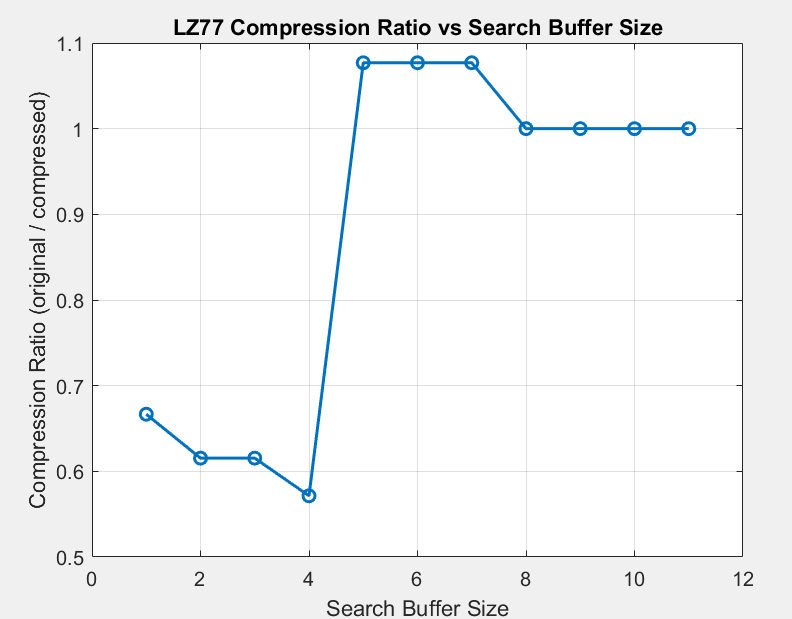
\includegraphics[width=\textwidth]{images/search-buffer-to-compression-ratio.png}
		\caption{Search Buffer vs Compression Ratio}
		\label{fig:search-buffer-compression-ratio}
	\end{subfigure}
	\hfill
	\begin{subfigure}{0.45\textwidth}
		\centering
		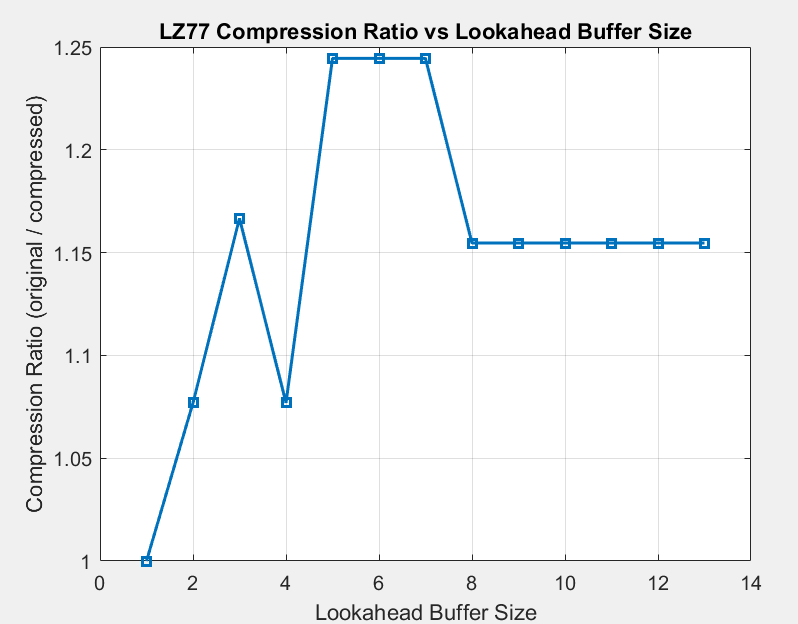
\includegraphics[width=\textwidth]{images/lookahead-buffer-to-compression-ratio.png}
		\caption{Look Ahead vs Compression Ratio}
		\label{fig:look-ahead-buffer-compression-ratio}
	\end{subfigure}
	\caption{Window Variation for Short Text}
	\label{fig:window-variation-short-text}
\end{figure}

Figure \ref{fig:window-variation-short-text} shows the results of this analysis. 
It can be seen that the variation is not some standard increase or decrease based on window size, but rather has a maxima and minima. 

A buffer length that is too small results in the algorithm being unable to efficiently set up it's pairs and dictionary, while one that's too long identifies redundantly long strings which messes up encoding.

However, this is only for the short string INKYPINKYPONKY. The same analysis was performed on the longer string.

\begin{figure}[htbp]
	\centering
	\begin{subfigure}{0.45\textwidth}
		\centering
		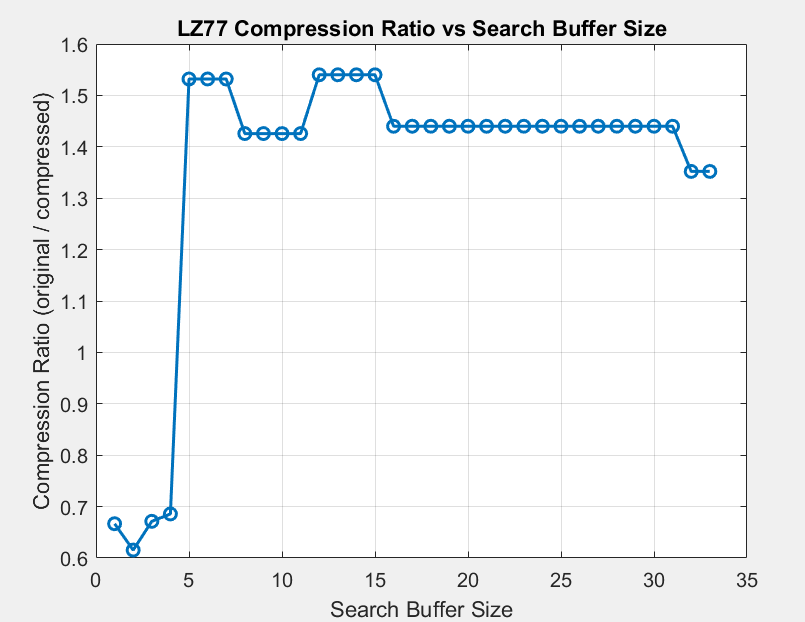
\includegraphics[width=\textwidth]{images/search-buffer-to-compression-ratio-longer.png}
		\caption{Search Buffer vs Compression Ratio}
		\label{fig:search-buffer-compression-ratio-long}
	\end{subfigure}
	\hfill
	\begin{subfigure}{0.45\textwidth}
		\centering
		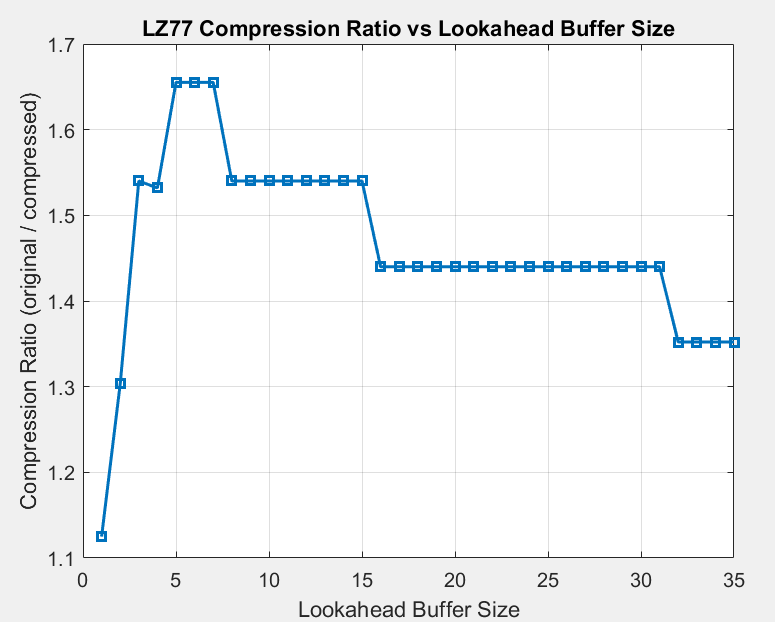
\includegraphics[width=\textwidth]{images/lookahead-buffer-to-compression-ratio-longer.png}
		\caption{Look Ahead vs Compression Ratio}
		\label{fig:look-ahead-buffer-compression-ratio-long}
	\end{subfigure}
	\caption{Window Variation for Longer Text}
	\label{fig:window-variation-long-text}
\end{figure}


\subsection{LZ78 Compression}
\label{subsec:lz78}
Unlike LZ77, LZ78 builds a dictionary of previously seen substrings and then transmits just the pairs. The dictionary gets built up on the receiving end, allowing for complete reconstruction of a message with just LZ78 pairs.

Code for the LZ78 compression function was implemented in MATLAB, and can be found in Appendix \ref{subappendix:lz78-code}. The resulting compressed pairs for the short string are as follows:

\begin{table}[h!]
	\centering
	\begin{tabular}{cc}
		\toprule
		Index & Next Character \\
		\midrule
		0 & I \\
		0 & N \\
		0 & K \\
		0 & Y \\
		0 & P \\
		1 & N \\
		3 & Y \\
		5 & O \\
		2 & K \\
		4 & EOF \\
		\bottomrule
	\end{tabular}
	\caption{LZ78 Compressed Pairs for Short String}
	\label{tab:lz78-pairs}
\end{table}

Since the dictionary doesn't have to be sent, we can use 3 bits for the index, and 8 bits for the literal. As such, the total number of compressed bits is:
\begin{align}
	3 * 10 + 8 * 9 = 102 \text{ bits}
\end{align}

This results in a \textbf{compression ratio of 1.098}.

The same was done with the longer string, and a compression ratio of 1.385 was achieved. 

\subsection{LZW Compression}
\label{subsec:lzw}
LZW compression is an extension of LZ78, where the dictionary is built dynamically and substrings are represented by indices in the dictionary. The initial dictionary contains all possible single-character strings.

The basic dictionary of LZW does cause a greater number of bits to be transmitted, but it's still sufficiently small to be manageable as it's only a few characters.

For LZW, there are three distinct pieces, the triplets (with the code, current char and next char), the dictionary, and the code stream. We only transmit the code stream and dictionary, which allows us to conserve bits.

For INKYPINKYPONKY, the following are the triplets:
\begin{table}[h!]
	\centering
	\begin{tabular}{ccc}
		\toprule
		Code & Current Character & Next Character \\
		\midrule
		1 & I & N \\
		2 & N & K \\
		3 & K & Y \\
		4 & Y & P \\
		5 & P & I \\
		7 & IN & K \\
		9 & KY & P \\
		5 & P & O \\
		6 & O & N \\
		7 & NK & Y \\
		4 & Y & EOF \\
		\bottomrule
	\end{tabular}
	\caption{LZW Triplets for Short String}
	\label{tab:lzw-triplets}
\end{table}

The dictionary that will be sent is only the basic part, as follows
\begin{center}
  1 → I,
  2 → N,
  3 → K,
  4 → Y,
  5 → P,
  6 → O
\end{center}

This results in 48 dictionary bits and 44 code bits, giving us 92 sent bits. The compression ratio is thus 1.217.

For the longer string, we end up with even better compression, with only 143 bits being sent, we get a compression ratio of 2.014.

\subsection{Summary of Text Compression Results}
\label{subsec:text-compression-summary}
The results of the text compression algorithms are summarized in Table \ref{tab:text-compression-summary}.
\begin{table}[h!]
	\centering
	\begin{tabular}{lcc}
		\toprule
		Algorithm & Compressed Bits & Compression Ratio \\
		\midrule
		LZ77 & 104 & 1.077 \\
		LZ78 & 102 & 1.098 \\
		LZW & 92 & 1.217 \\
		\bottomrule
	\end{tabular}
	\caption{Summary of Text Compression Results (Short String)}
	\label{tab:text-compression-summary}
\end{table}

It's clear that LZW performed the best for the given string, and it's of no doubt as it best transmits the data, with just coded bits and the overhead for the basic dictionary.

Additionally, LZ77 is highly dependent on window size as discussed in Section \ref{subsubsec:lz77-window-size}, and thus may perform better or worse based on the window size chosen, but for the given parameters, it did not. Code for LZ77 decompression is provided in Appendix \ref{subappendix:lz77-decompress-code}.

\section{Image Compression}
\label{sec:image-compression}
The second part of the assignment involved implementing three different image compression algorithms: Block Transform Coding (BTC), Predictive Coding (DPCM), and Wavelet Coding (DWT). These algorithms were tested on four images derived from the previous assignments.

The four test images consisted of:
\begin{itemize}
	\item Image 1: Grayscale version of Assignment 1 image
	\item Image 2: Binary version of Assignment 1 image  
	\item Image 3: Grayscale version of Assignment 2 image
	\item Image 4: Binary version of Assignment 2 image
\end{itemize}

All compression algorithms used a patch size of $16 \times 16$ pixels and a quantization parameter $Q = 5$ for grayscale images.

\subsection{Block Transform Coding}
\label{subsec:block-transform-coding}
Block Transform Coding (BTC) is a lossy compression technique that divides an image into fixed-size blocks and applies a transform to each block. In this implementation, the Discrete Cosine Transform (DCT) was used.

\subsubsection{Algorithm Overview}
The BTC algorithm consists of the following steps:
\begin{enumerate}
	\item Divide the input image into non-overlapping blocks of size $16 \times 16$
	\item Apply 2D DCT to each block
	\item Quantize the DCT coefficients using scalar quantization with step size $Q$
	\item Encode the quantized coefficients using zig-zag scanning
	\item Estimate the compressed size using entropy coding principles
\end{enumerate}

For decompression, the inverse process is applied: dequantize the coefficients and apply inverse DCT (IDCT) to reconstruct each block.

The zig-zag scan ordering ensures that low-frequency components (which contain most of the image energy) are placed first in the sequence, allowing for more efficient encoding.

\subsubsection{Results}
The BTC algorithm achieved varying compression ratios across different image types. The complete code implementation is provided in Appendix \ref{subappendix:btc-code}.

\begin{table}[h!]
	\centering
	\begin{tabular}{lccc}
		\toprule
		Image & Compression Ratio & MSE & PSNR (dB) \\
		\midrule
		Image 1 Grayscale & 5.640 & 1.26 & 46.86 \\
		Image 1 Binary & 6.311 & 0.14 & 56.53 \\
		Image 2 Grayscale & 4.970 & 0.87 & 48.38 \\
		Image 2 Binary & 3.504 & 0.30 & 53.12 \\
		\bottomrule
	\end{tabular}
	\caption{Block Transform Coding Results}
	\label{tab:btc-results}
\end{table}

As shown in Table \ref{tab:btc-results}, BTC performed exceptionally well on binary images from Assignment 1 (Image 1 Binary), achieving the highest compression ratio of 6.311 with minimal quality loss (PSNR = 56.53 dB).

\subsection{Predictive Coding (DPCM)}
\label{subsec:predictive-coding}
Differential Pulse Code Modulation (DPCM) is a predictive coding technique that exploits spatial correlation in images. Instead of encoding pixel values directly, DPCM encodes the difference between the actual pixel value and a predicted value based on neighboring pixels.

\subsubsection{Algorithm Overview}
The DPCM algorithm uses the following prediction rules:
\begin{itemize}
	\item \textbf{Top-left corner} (i=1, j=1): Prediction = 0
	\item \textbf{First column} (j=1): Prediction = pixel above
	\item \textbf{First row} (i=1): Prediction = pixel to the left
	\item \textbf{All other pixels}: Prediction = average of pixel above and pixel to the left
\end{itemize}

The compression process is as follows:
\begin{enumerate}
	\item Quantize the original image with step size $Q$
	\item Compute predicted values using the rules above
	\item Calculate prediction errors: $e(i,j) = \text{actual}(i,j) - \text{predicted}(i,j)$
	\item Quantize and encode the error values
\end{enumerate}

For decompression, the image is reconstructed by adding the quantized errors back to the predicted values.

\subsubsection{Results}
The DPCM implementation achieved consistent but moderate compression ratios across all test images.

\begin{table}[h!]
	\centering
	\begin{tabular}{lccc}
		\toprule
		Image & Compression Ratio & MSE & PSNR (dB) \\
		\midrule
		Image 1 Grayscale & 2.000 & 9.08 & 38.51 \\
		Image 1 Binary & 1.600 & 0.17 & 55.79 \\
		Image 2 Grayscale & 2.000 & 15.58 & 36.19 \\
		Image 2 Binary & 1.600 & 0.26 & 53.86 \\
		\bottomrule
	\end{tabular}
	\caption{Predictive Coding (DPCM) Results}
	\label{tab:dpcm-results}
\end{table}

As evident from Table \ref{tab:dpcm-results}, DPCM showed the most consistent behavior across different image types, with compression ratios of approximately 2.0 for grayscale images and 1.6 for binary images. The PSNR values for binary images remained high (>53 dB), indicating excellent reconstruction quality.

\subsection{Wavelet Coding}
\label{subsec:wavelet-coding}
Wavelet coding leverages the multi-resolution analysis capabilities of wavelet transforms. This implementation uses a simplified approach where only the low-low (LL) subband is retained after wavelet decomposition.

\subsubsection{Algorithm Overview}
The wavelet compression algorithm proceeds as follows:
\begin{enumerate}
	\item Quantize the input image with step size $Q$
	\item Apply 2D averaging-based wavelet transform
	\item Compute row-wise low-pass (averaging) operation
	\item Compute column-wise low-pass operation on the row-averaged result
	\item Retain only the LL (low-low frequency) subband
	\item Encode the LL coefficients
\end{enumerate}

For reconstruction, the LL subband is upsampled by replicating each coefficient to recover the original dimensions. This results in a smoothed approximation of the original image.

\subsubsection{Results}
The wavelet coding approach showed interesting behavior depending on image type.

\begin{table}[h!]
	\centering
	\begin{tabular}{lccc}
		\toprule
		Image & Compression Ratio & MSE & PSNR (dB) \\
		\midrule
		Image 1 Grayscale & 4.008 & 17.51 & 35.67 \\
		Image 1 Binary & 7.627 & 288.91 & 23.52 \\
		Image 2 Grayscale & 4.002 & 39.88 & 32.12 \\
		Image 2 Binary & 6.469 & 463.52 & 21.47 \\
		\bottomrule
	\end{tabular}
	\caption{Wavelet Coding (LL-only) Results}
	\label{tab:dwt-results}
\end{table}

Table \ref{tab:dwt-results} reveals a trade-off in wavelet coding: while it achieved the highest compression ratios for binary images (up to 7.627), this came at the cost of significant quality degradation (PSNR as low as 21.47 dB for Image 2 Binary).

\subsection{Visual Comparison}
\label{subsec:visual-comparison}
Figures \ref{fig:img1-gray-comparison} through \ref{fig:img2-bin-comparison} show the reconstructed images for all three compression methods across the four test images, with Figure \ref{fig:compression-comparison} providing a quantitative comparison.

\begin{figure}[p]
	\centering
	\begin{subfigure}[t]{0.23\textwidth}
		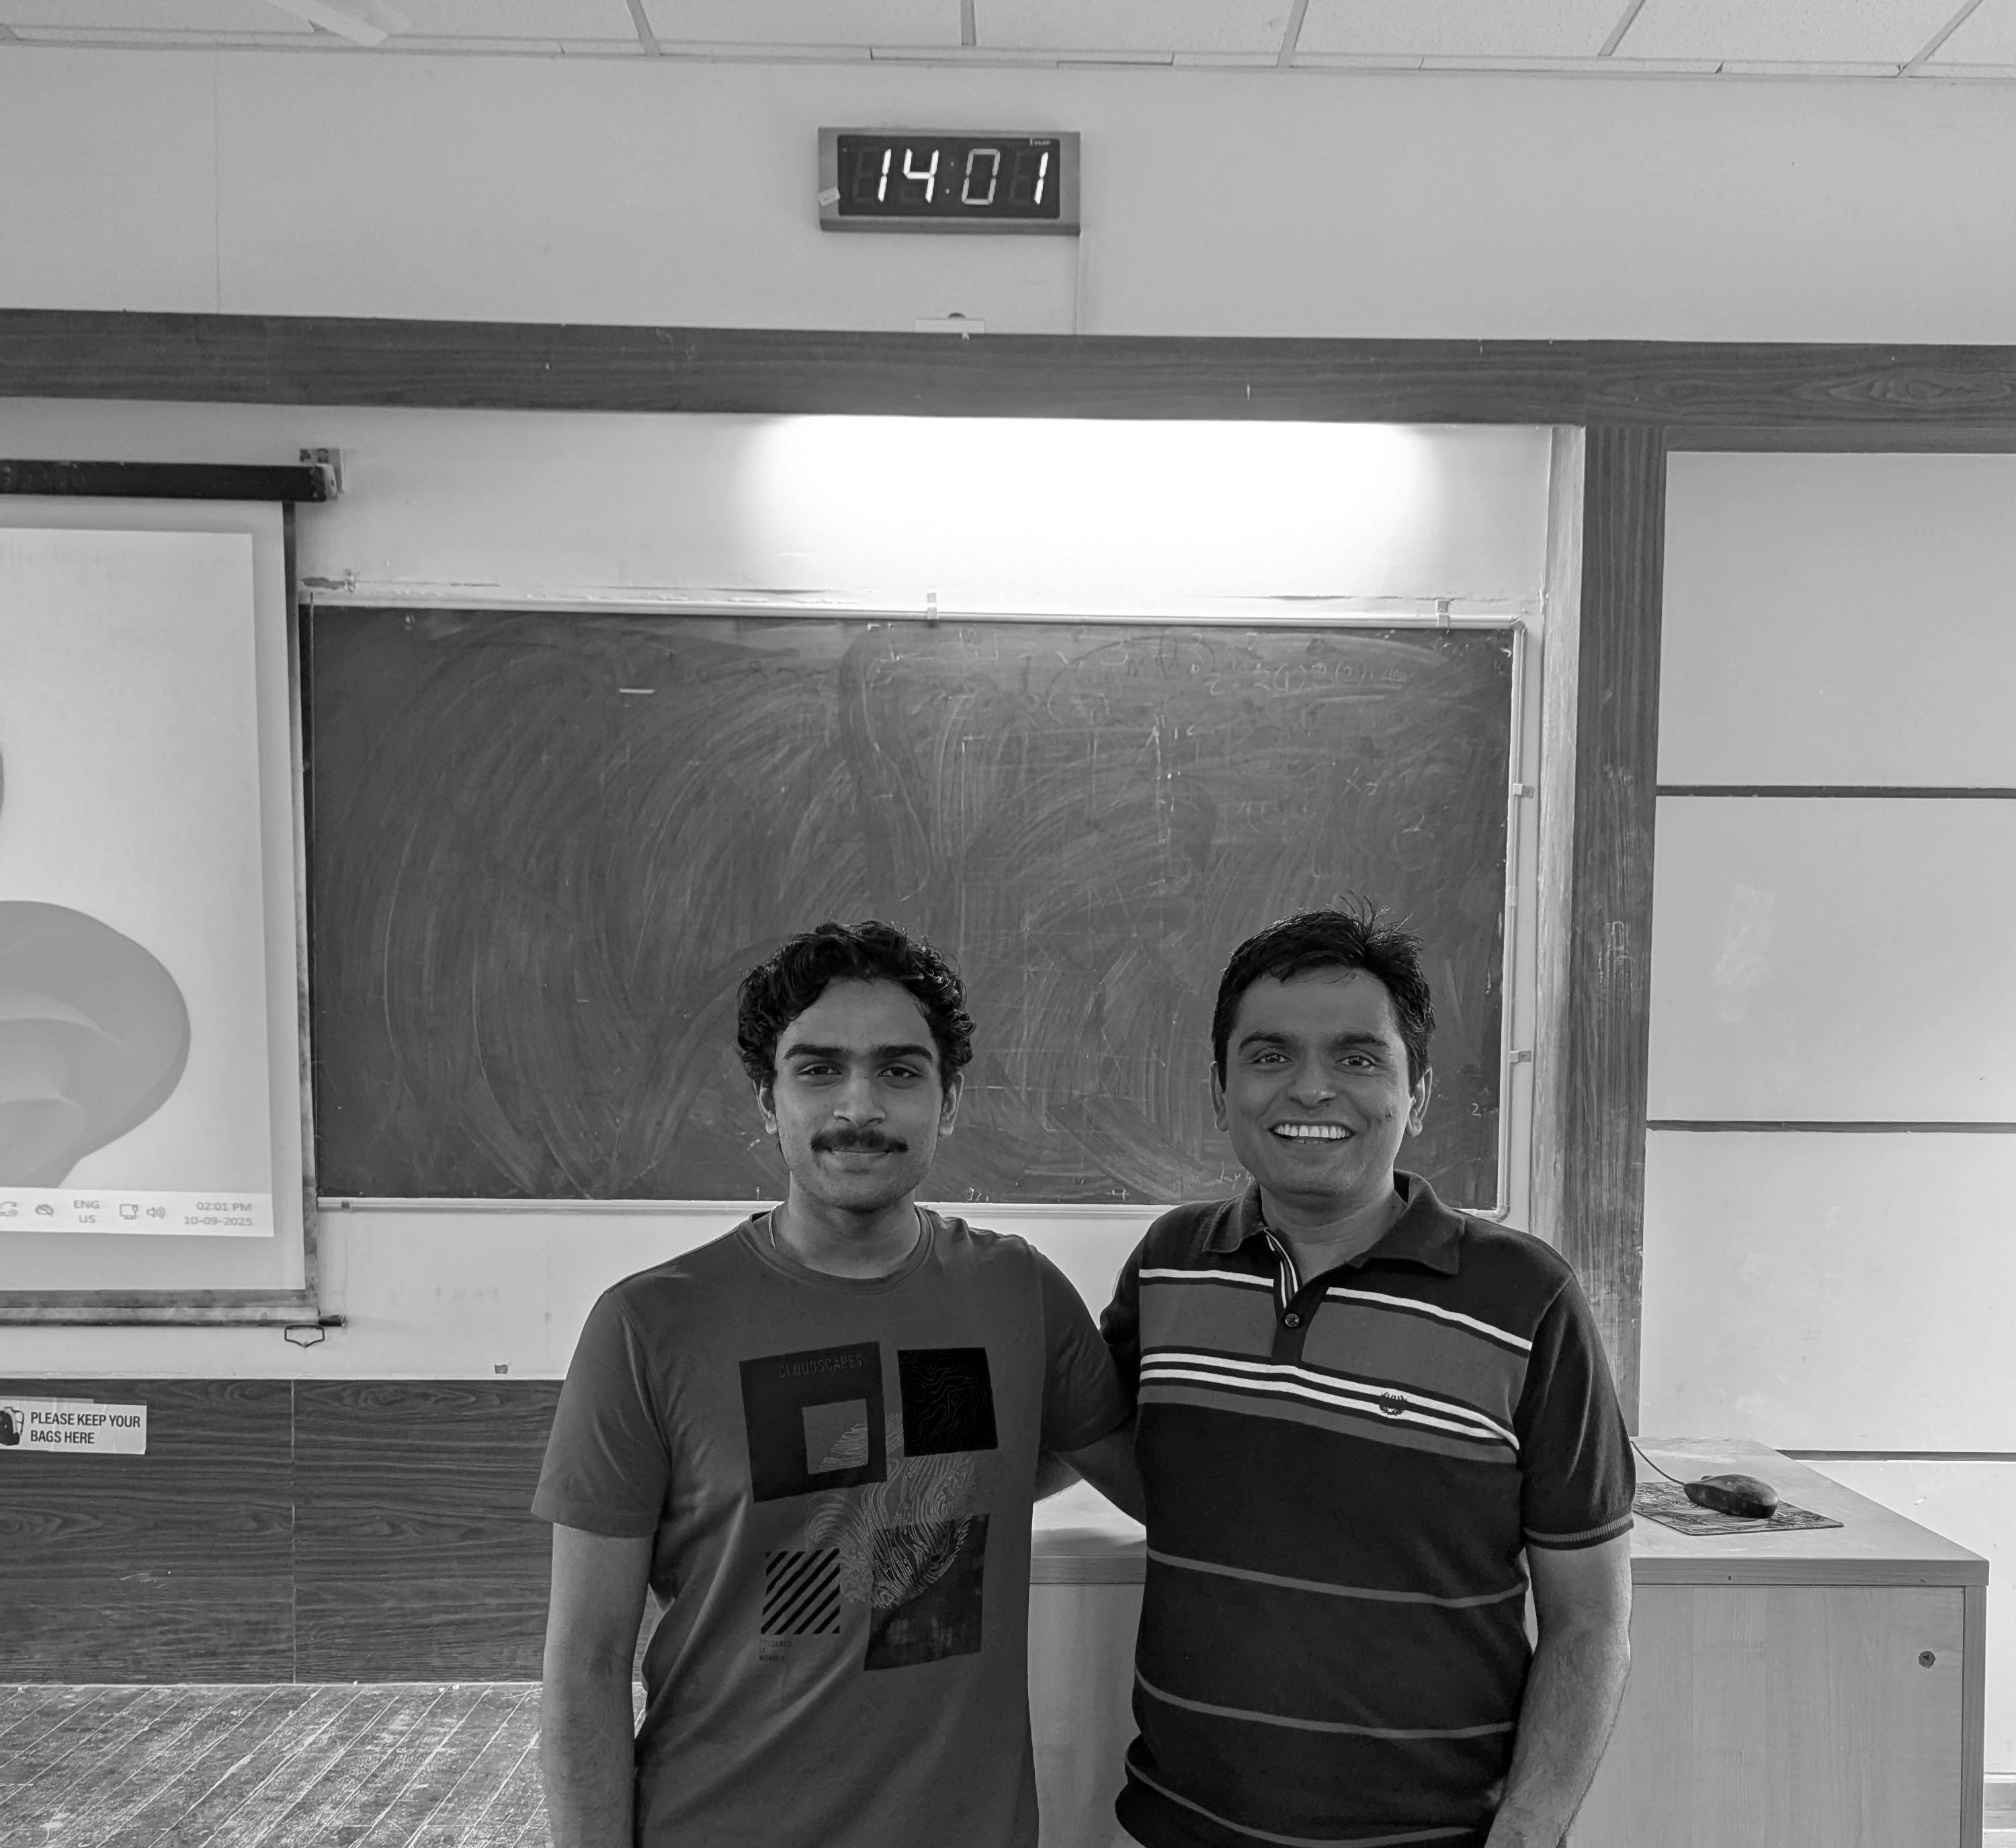
\includegraphics[width=\textwidth]{images/Image01_Original.png}
		\caption{Original}
	\end{subfigure}
	\hfill
	\begin{subfigure}[t]{0.23\textwidth}
		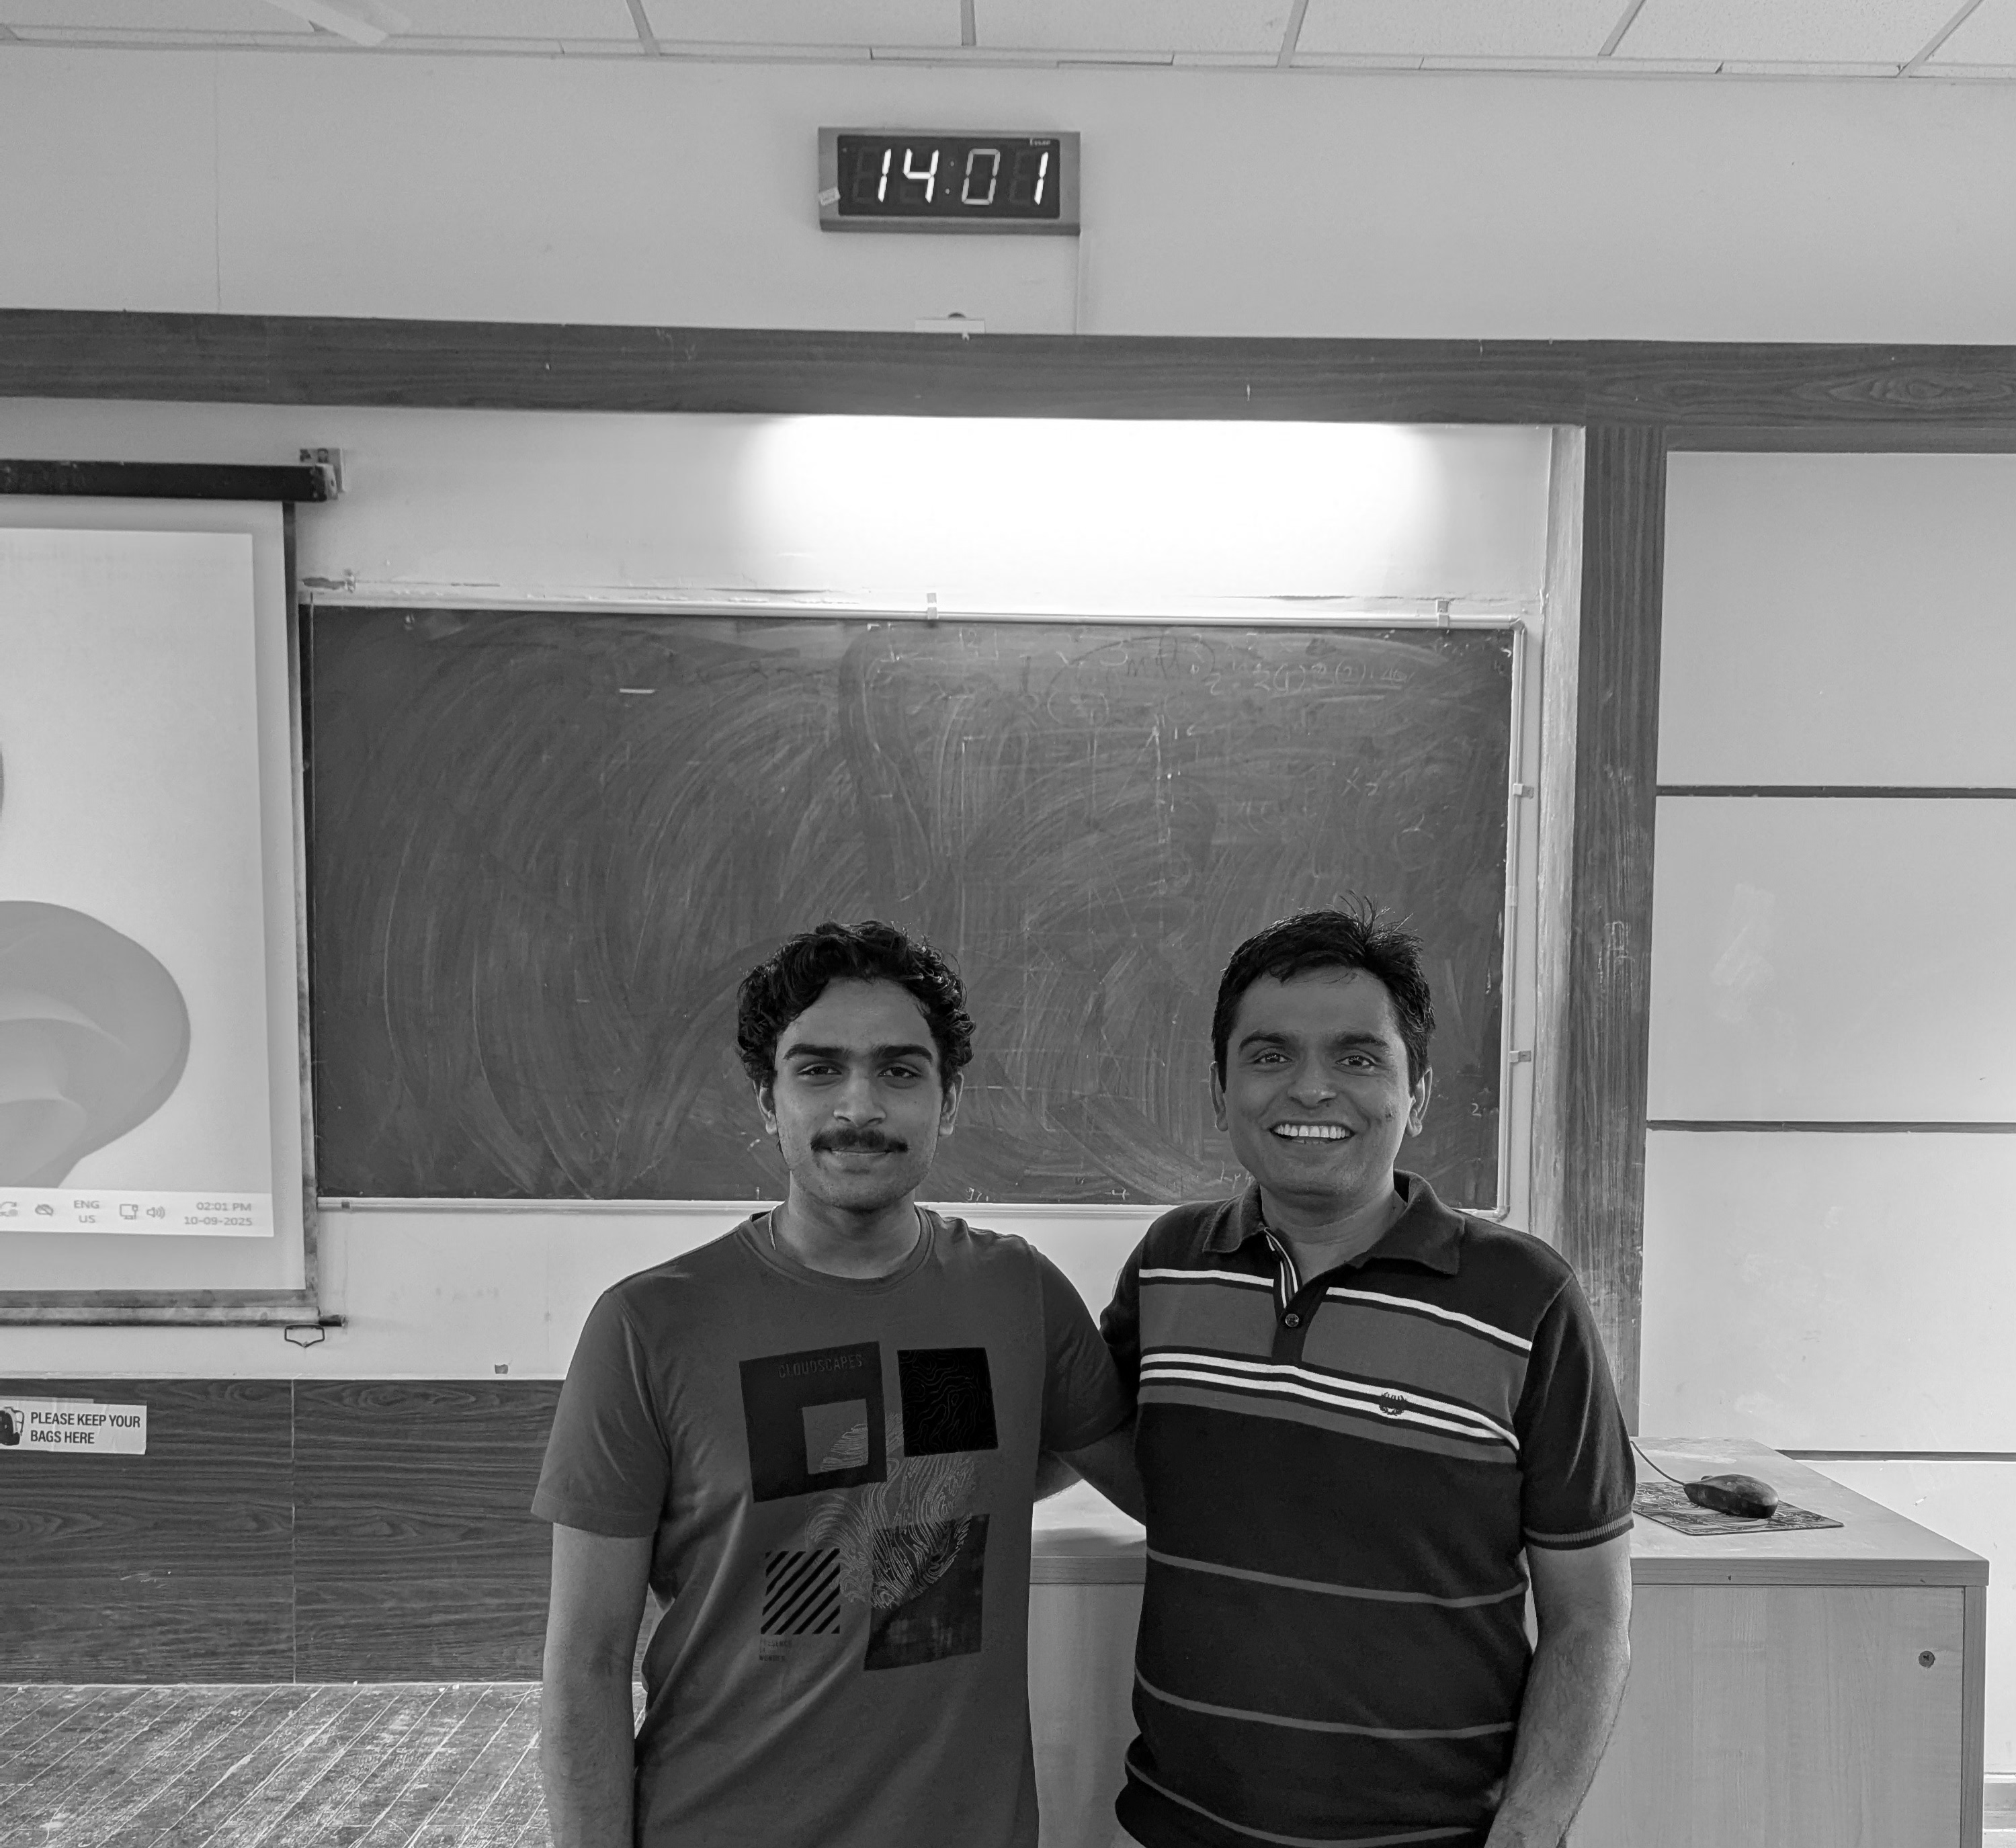
\includegraphics[width=\textwidth]{images/Image01_BTC.png}
		\caption{BTC}
	\end{subfigure}
	\hfill
	\begin{subfigure}[t]{0.23\textwidth}
		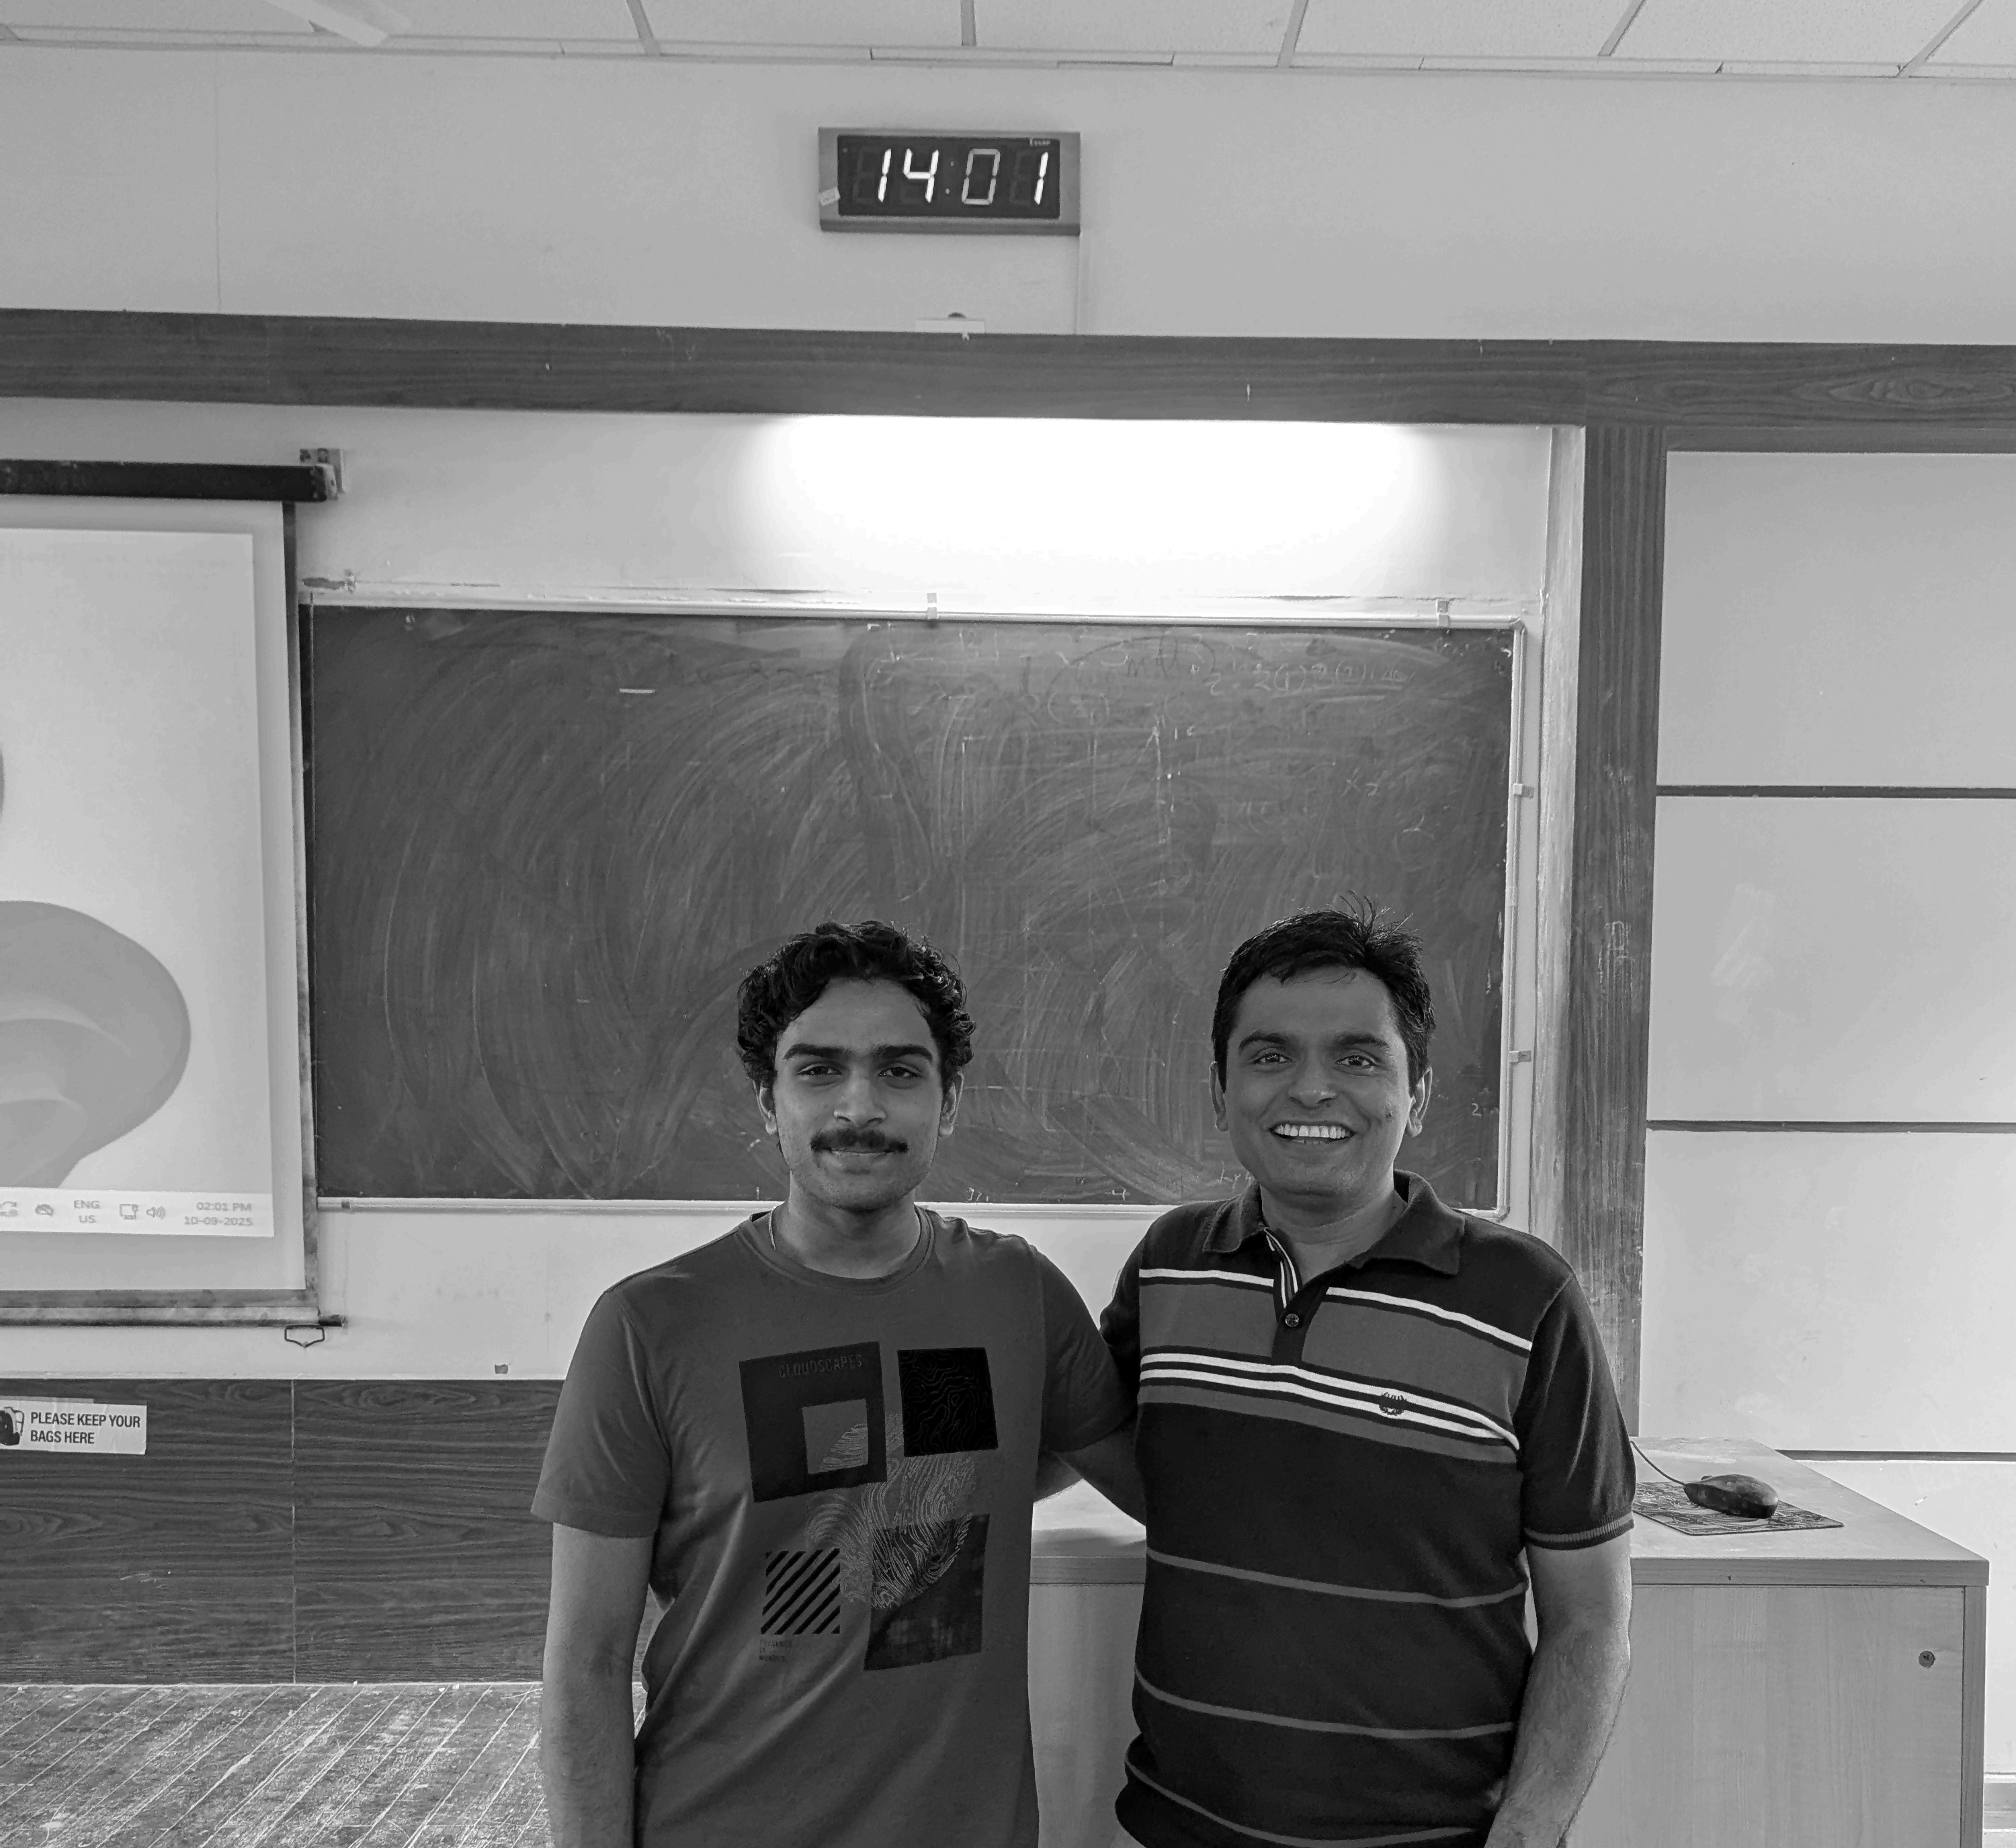
\includegraphics[width=\textwidth]{images/Image01_DPCM.png}
		\caption{DPCM}
	\end{subfigure}
	\hfill
	\begin{subfigure}[t]{0.23\textwidth}
		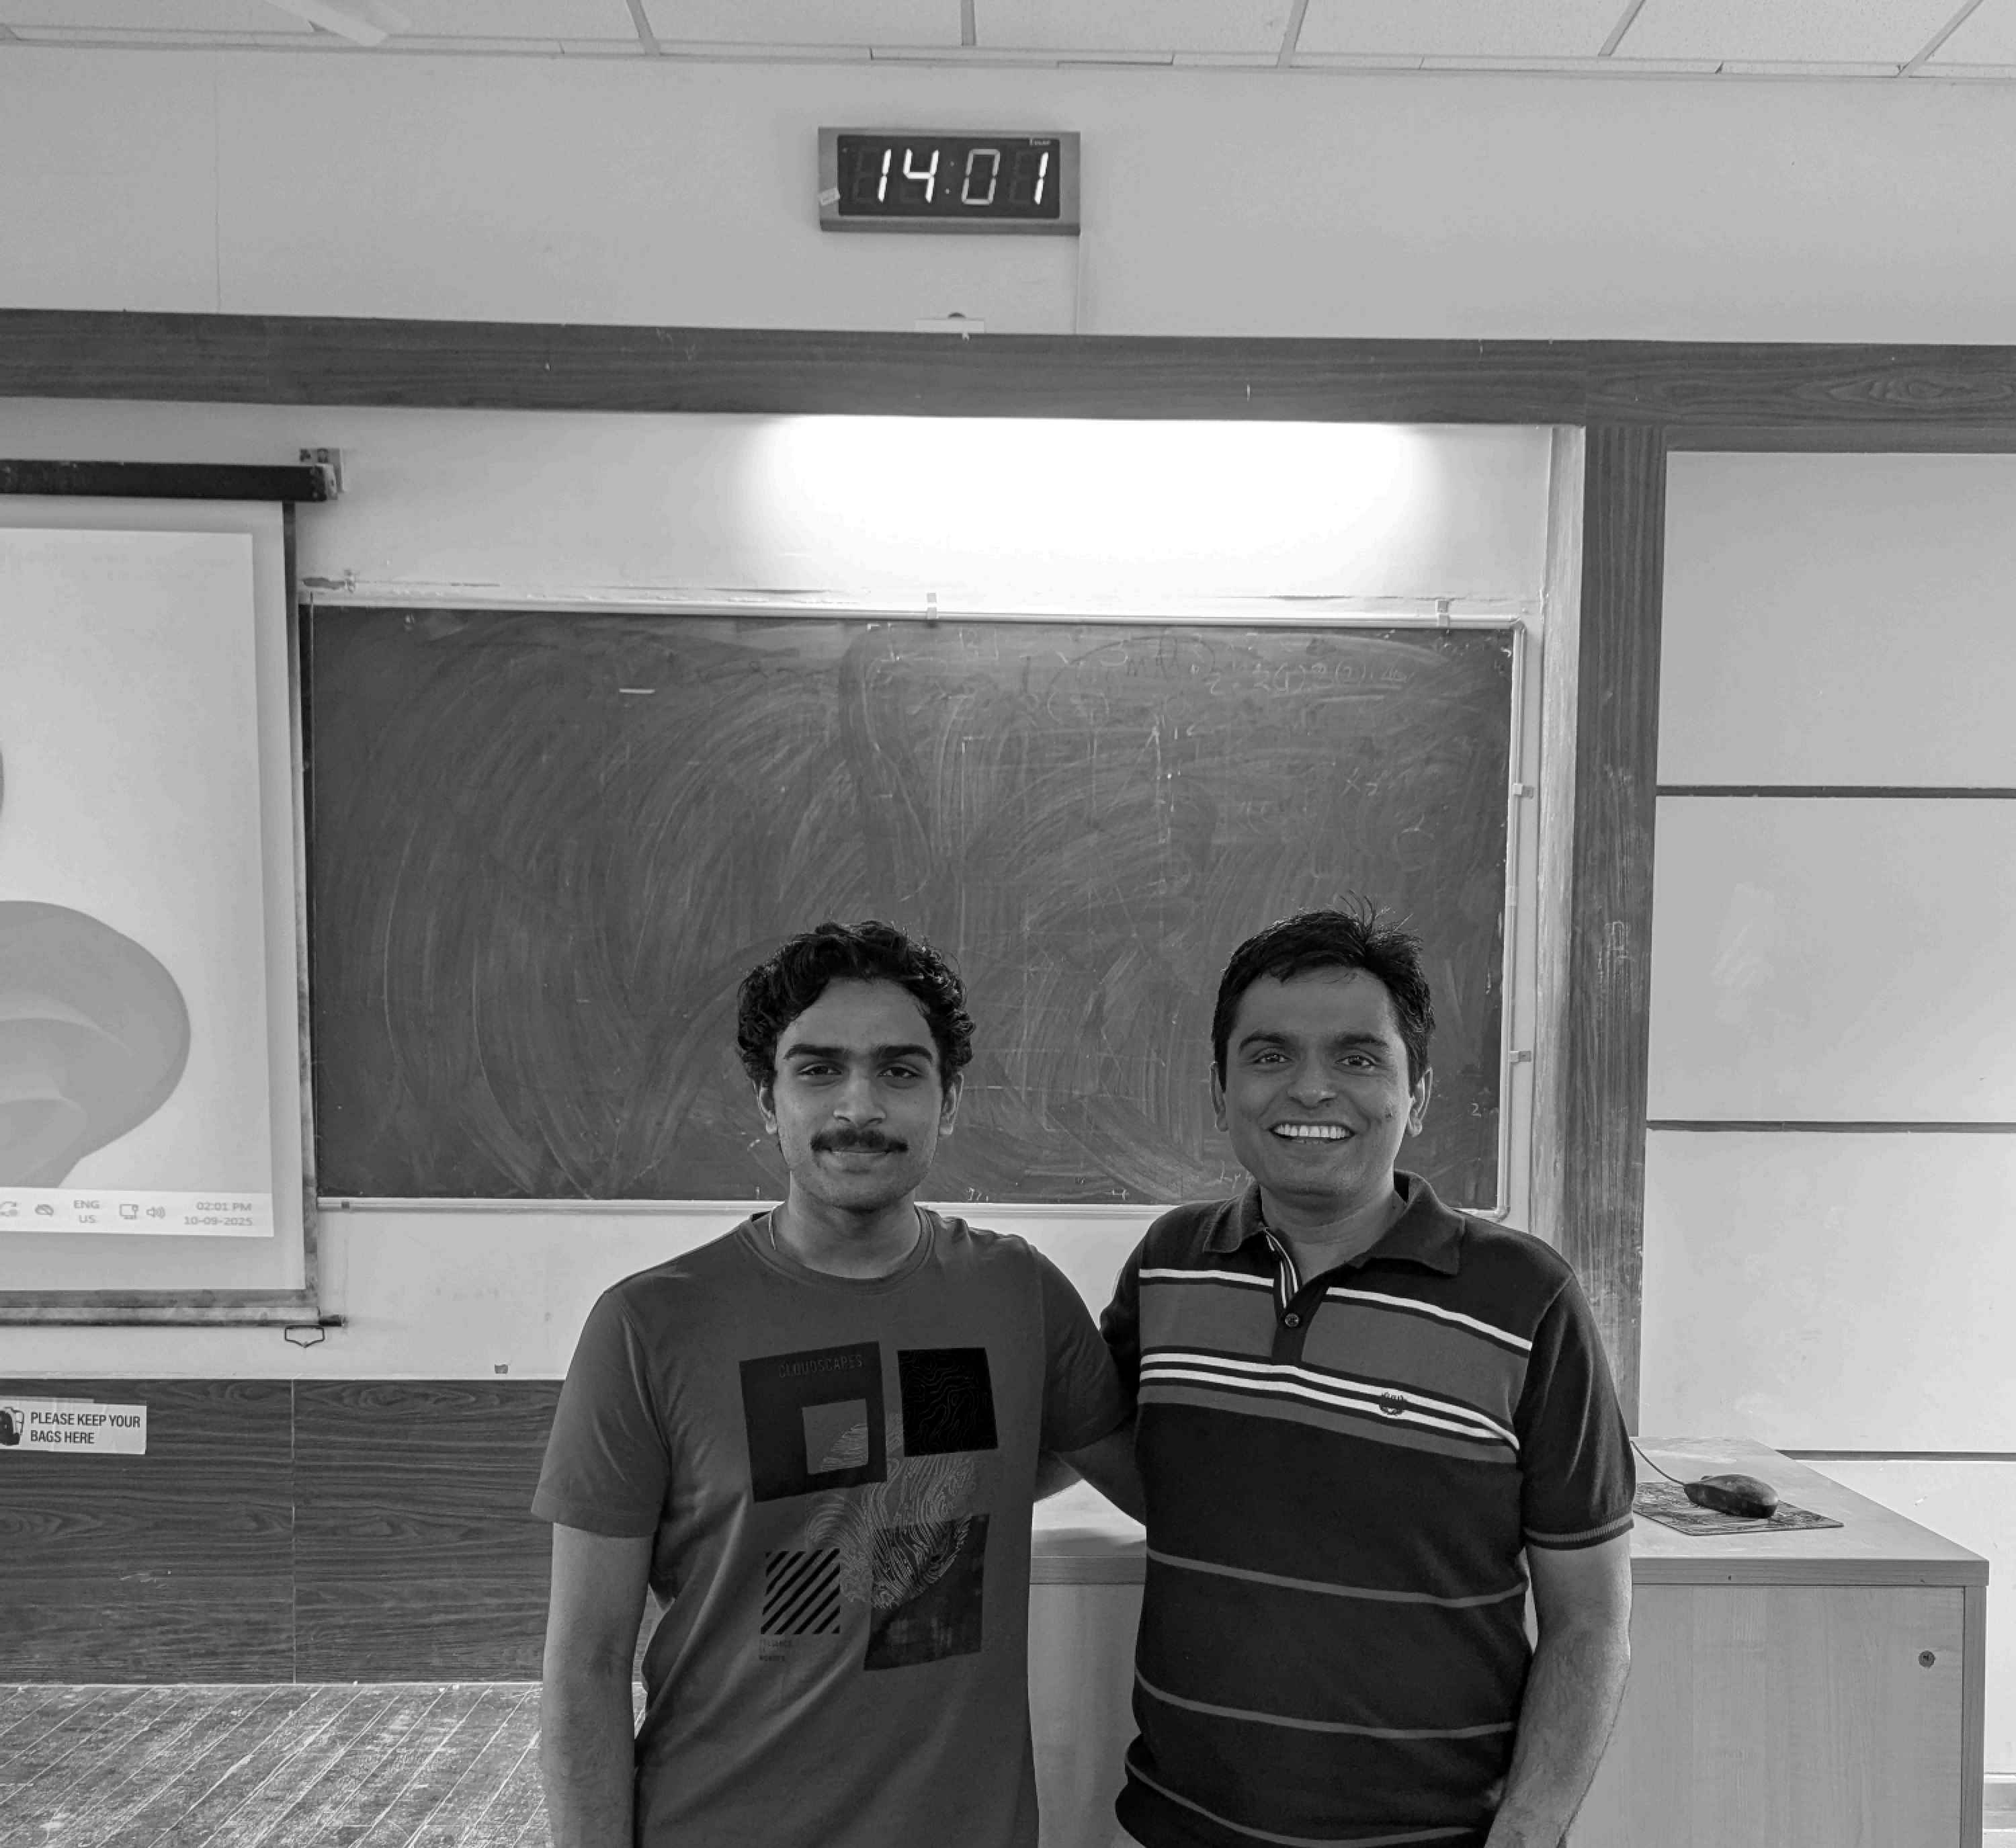
\includegraphics[width=\textwidth]{images/Image01_DWT.png}
		\caption{DWT}
	\end{subfigure}
	\caption{Image 1 Grayscale - Compression Comparison}
	\label{fig:img1-gray-comparison}
	
	\vspace{1.5cm}
	
	\begin{subfigure}[t]{0.23\textwidth}
		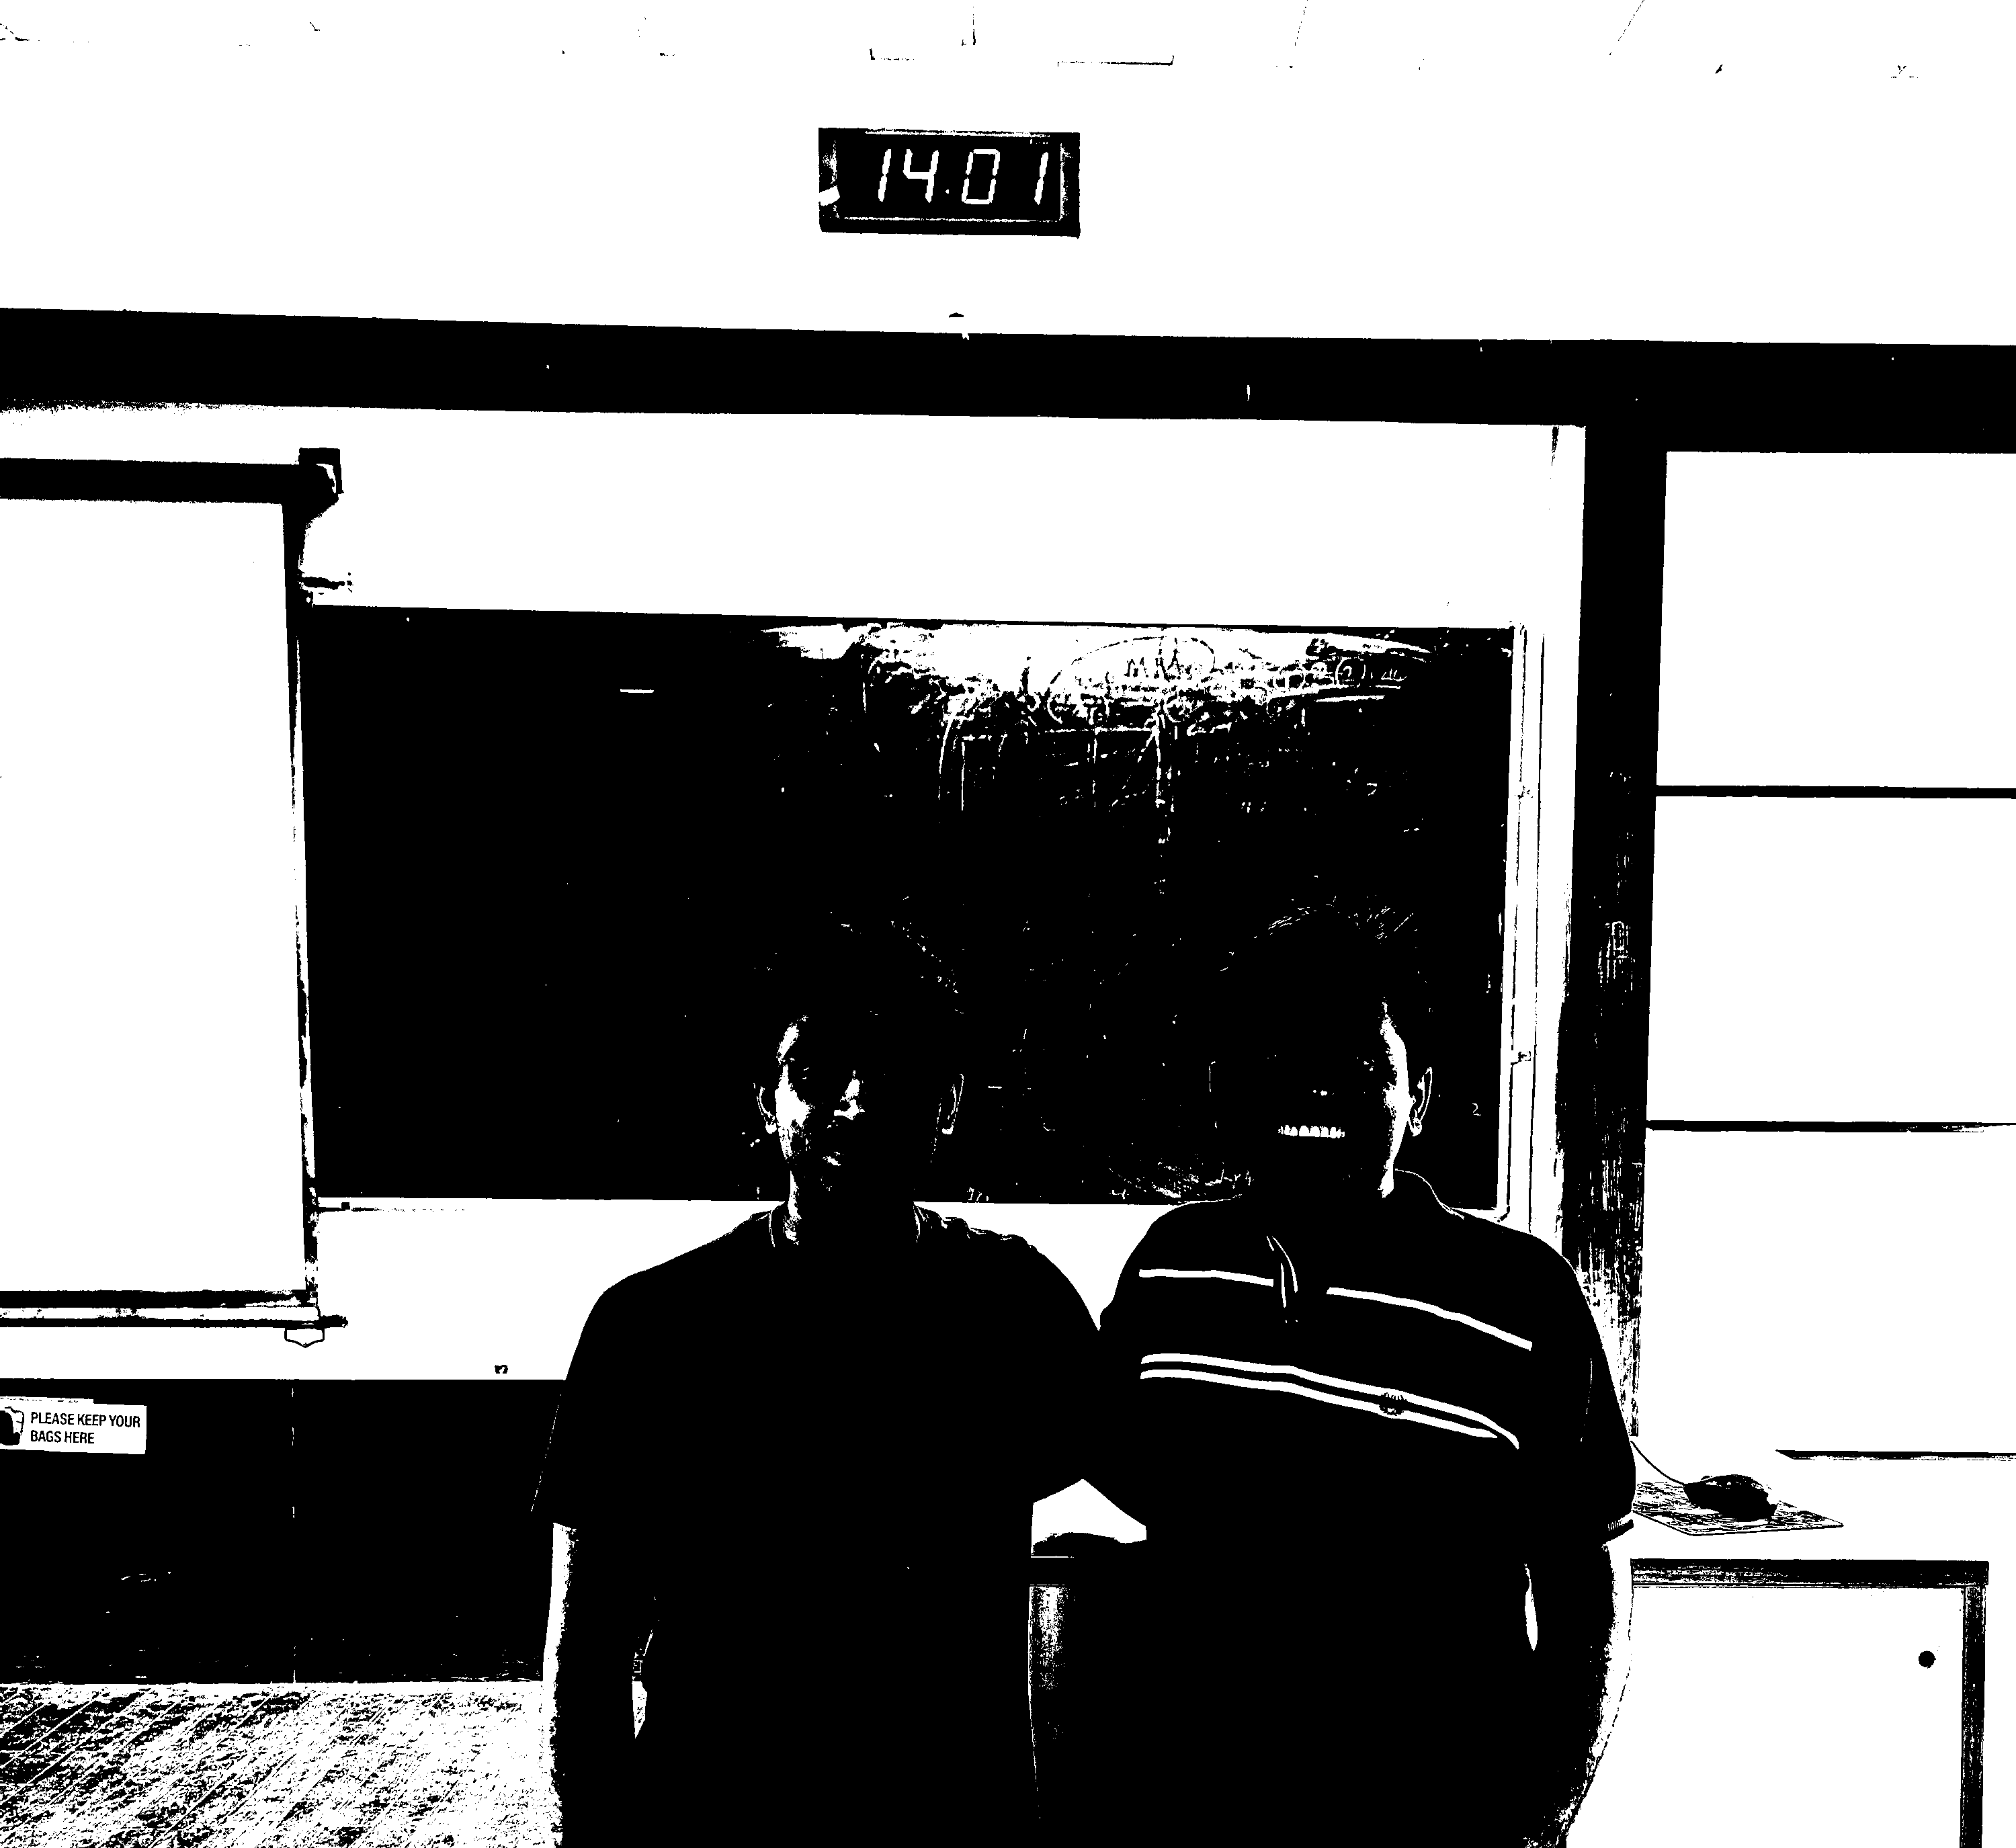
\includegraphics[width=\textwidth]{images/Image02_Original.png}
		\caption{Original}
	\end{subfigure}
	\hfill
	\begin{subfigure}[t]{0.23\textwidth}
		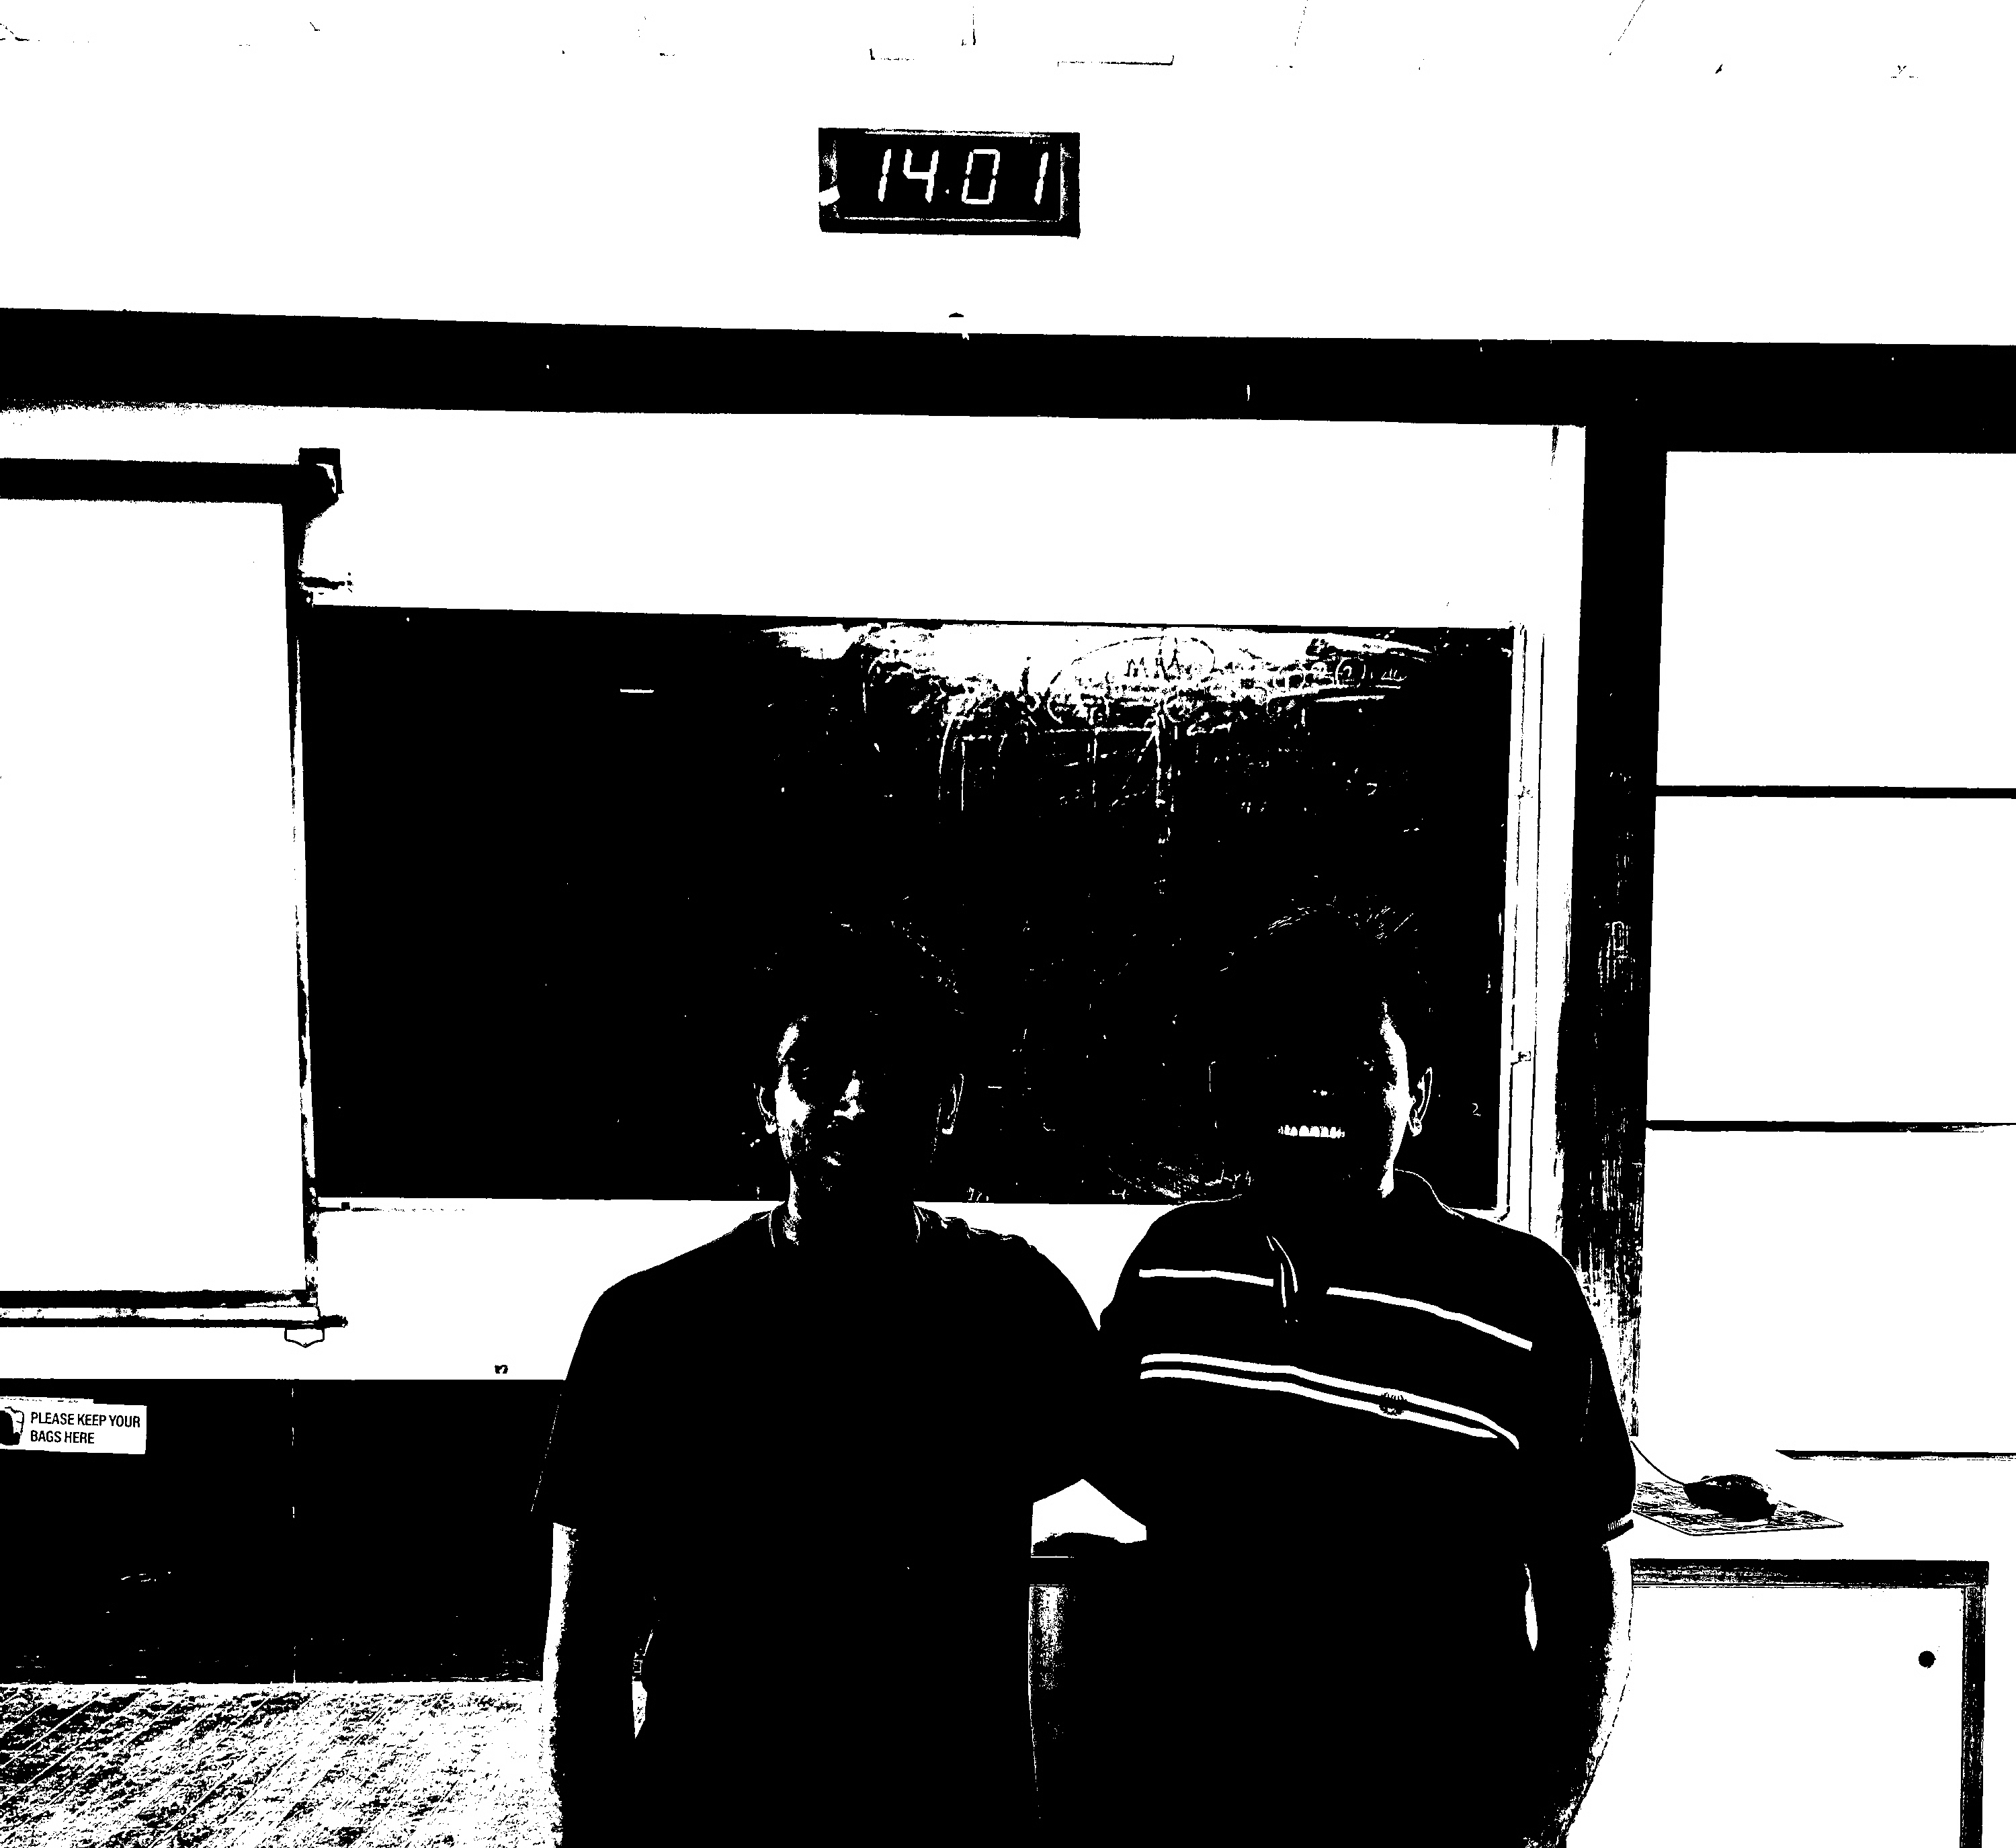
\includegraphics[width=\textwidth]{images/Image02_BTC.png}
		\caption{BTC}
	\end{subfigure}
	\hfill
	\begin{subfigure}[t]{0.23\textwidth}
		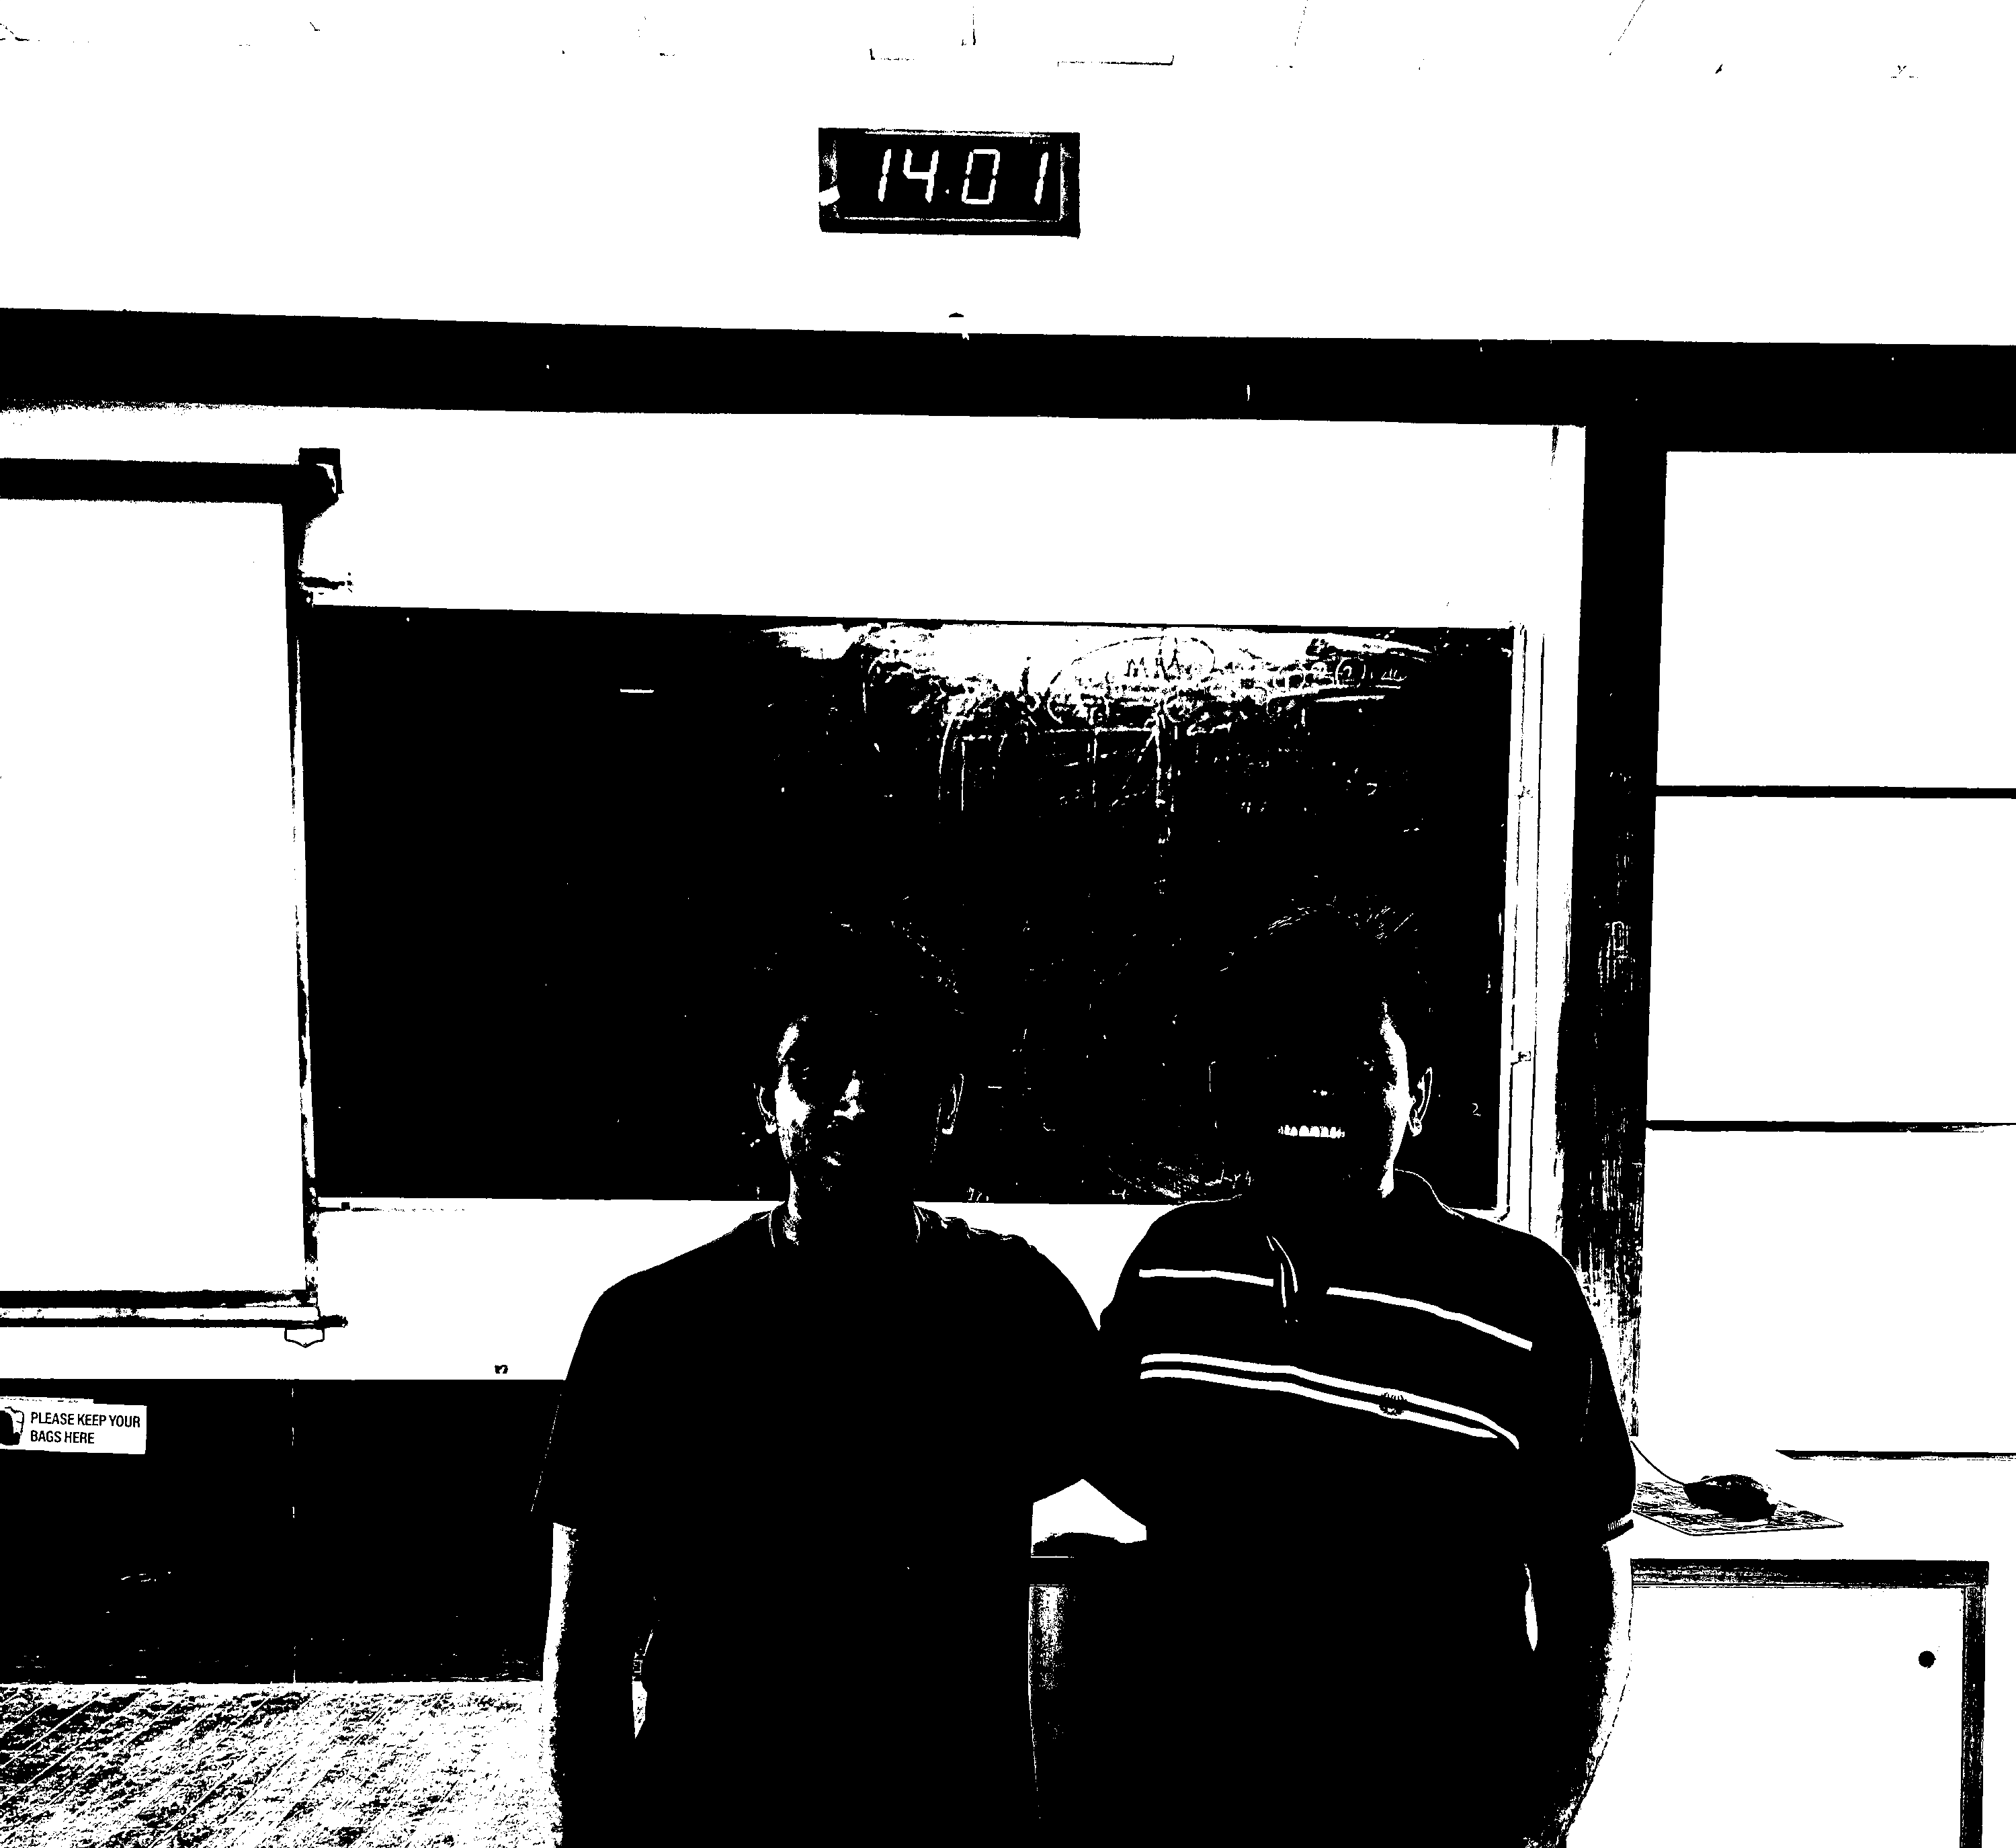
\includegraphics[width=\textwidth]{images/Image02_DPCM.png}
		\caption{DPCM}
	\end{subfigure}
	\hfill
	\begin{subfigure}[t]{0.23\textwidth}
		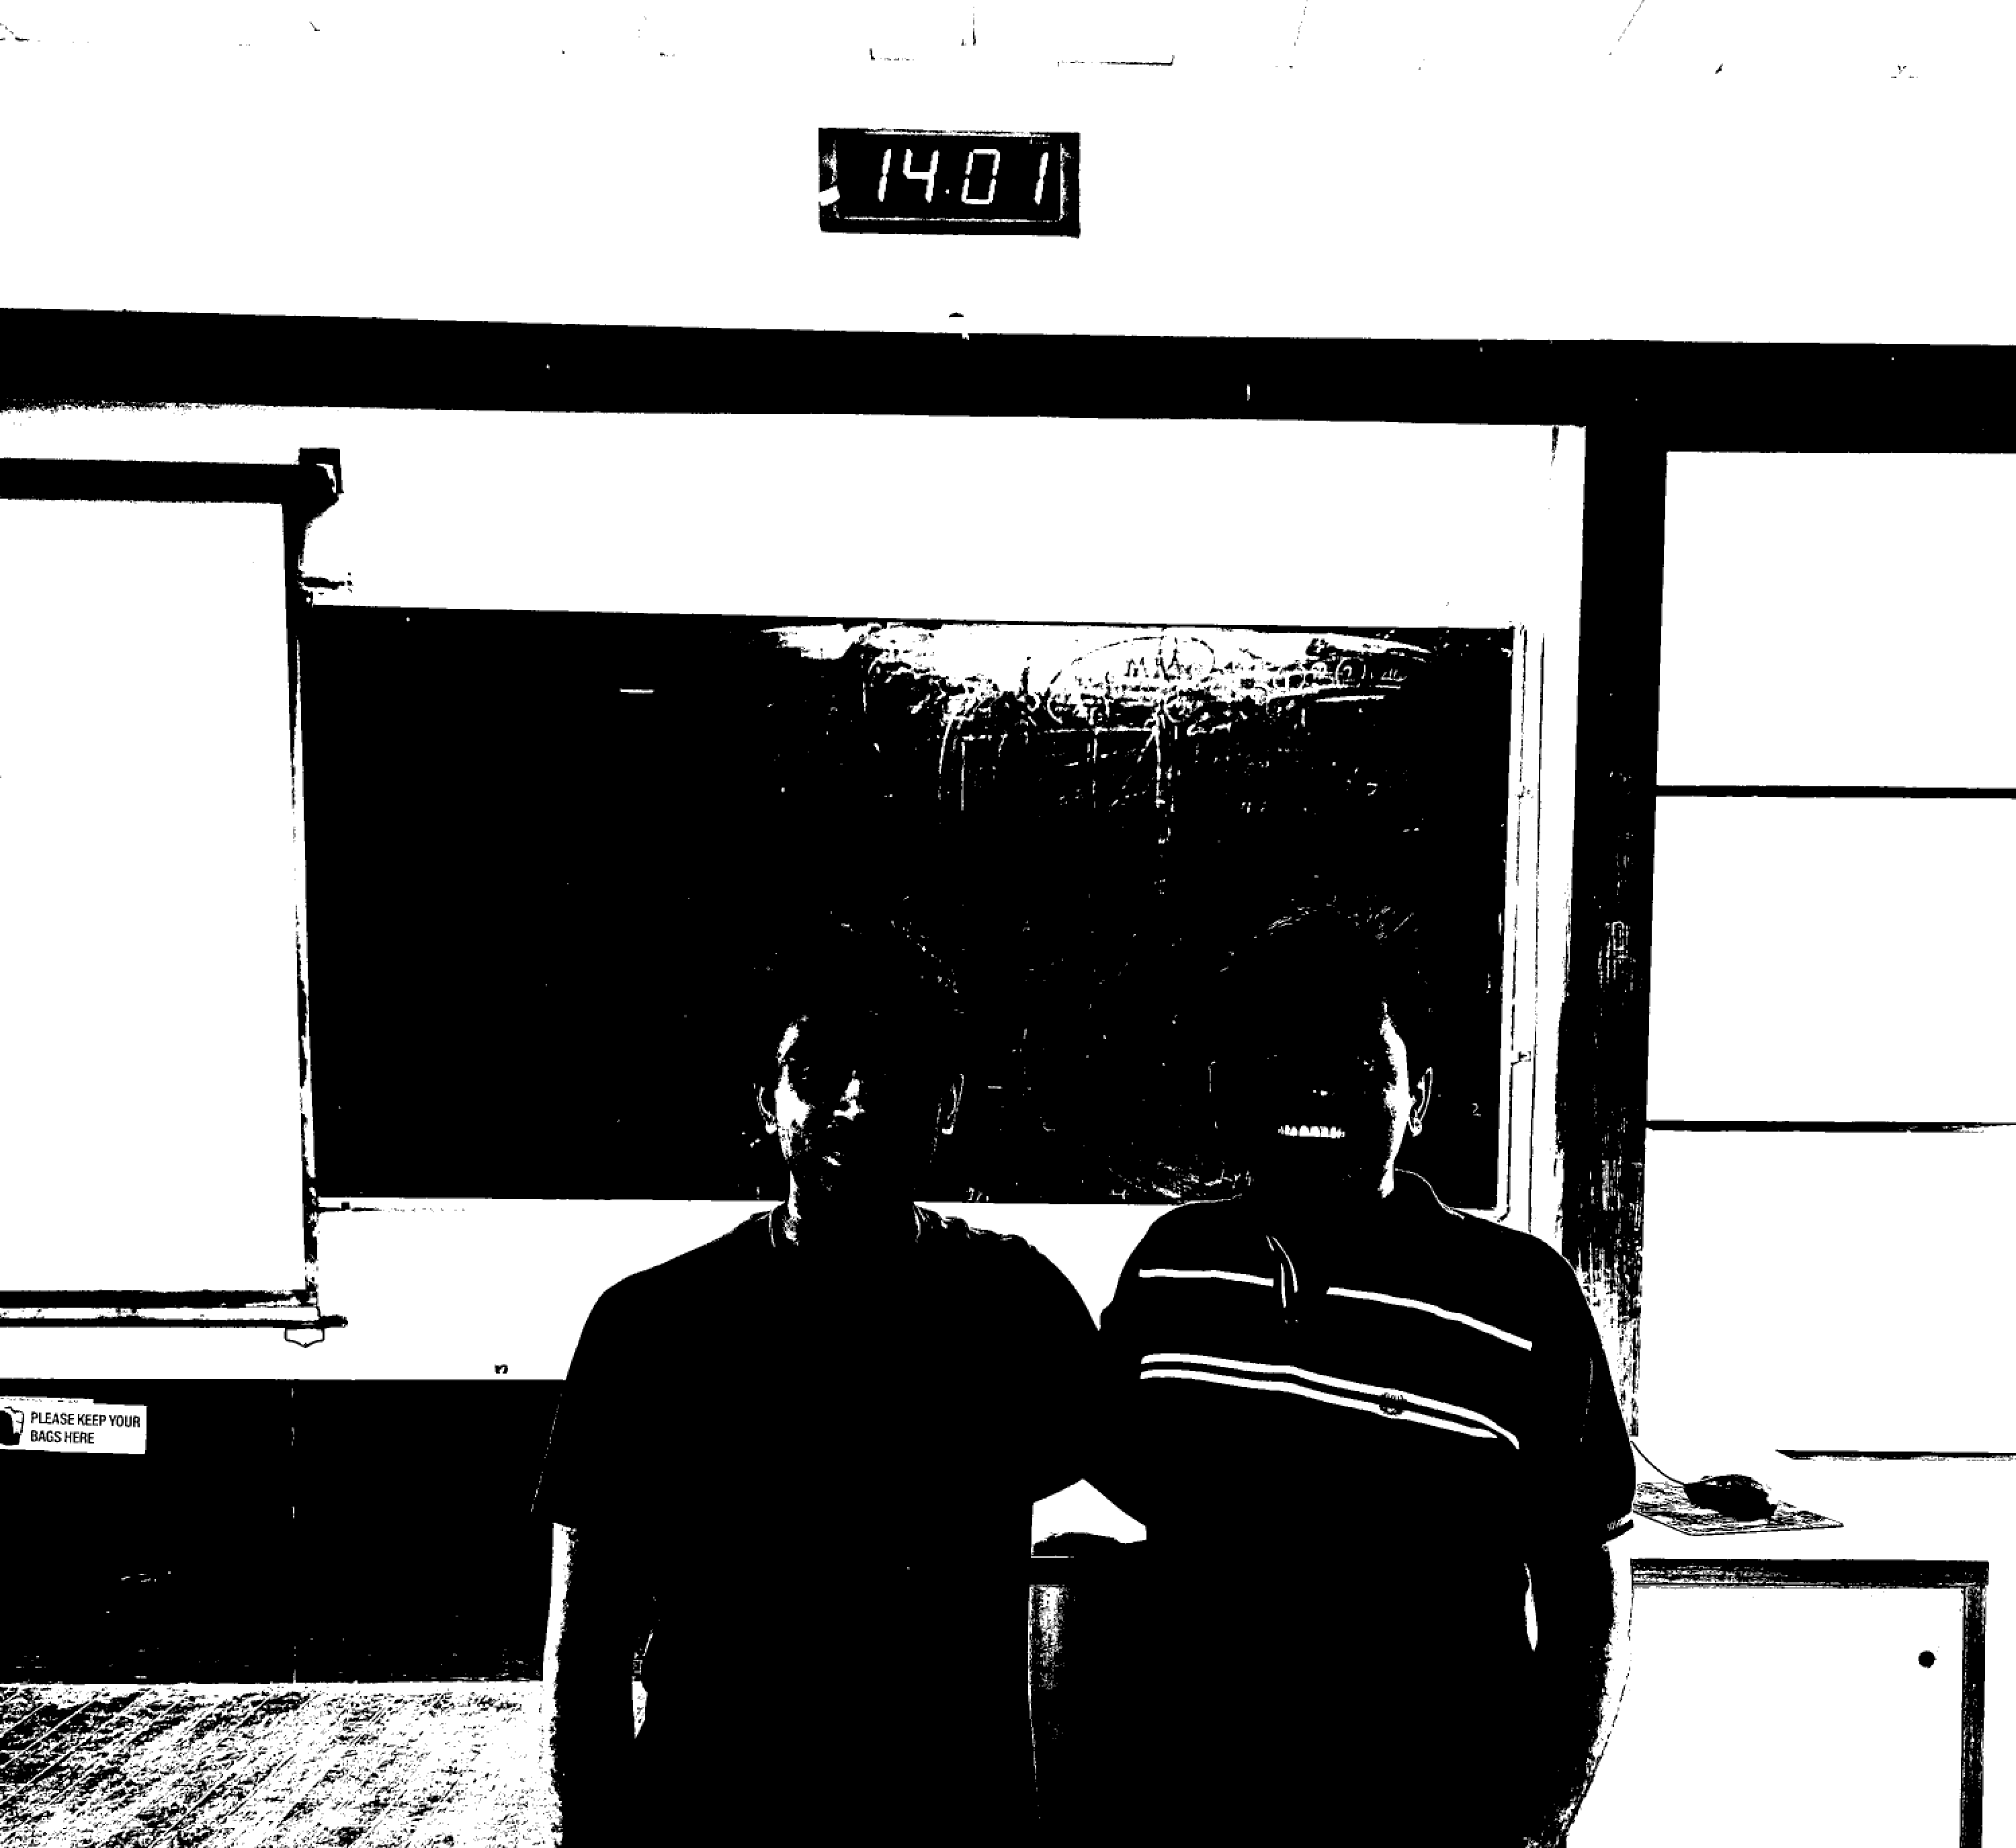
\includegraphics[width=\textwidth]{images/Image02_DWT.png}
		\caption{DWT}
	\end{subfigure}
	\caption{Image 1 Binary - Compression Comparison}
	\label{fig:img1-bin-comparison}
\end{figure}

\begin{figure}[p]
	\centering
	\begin{subfigure}[t]{0.23\textwidth}
		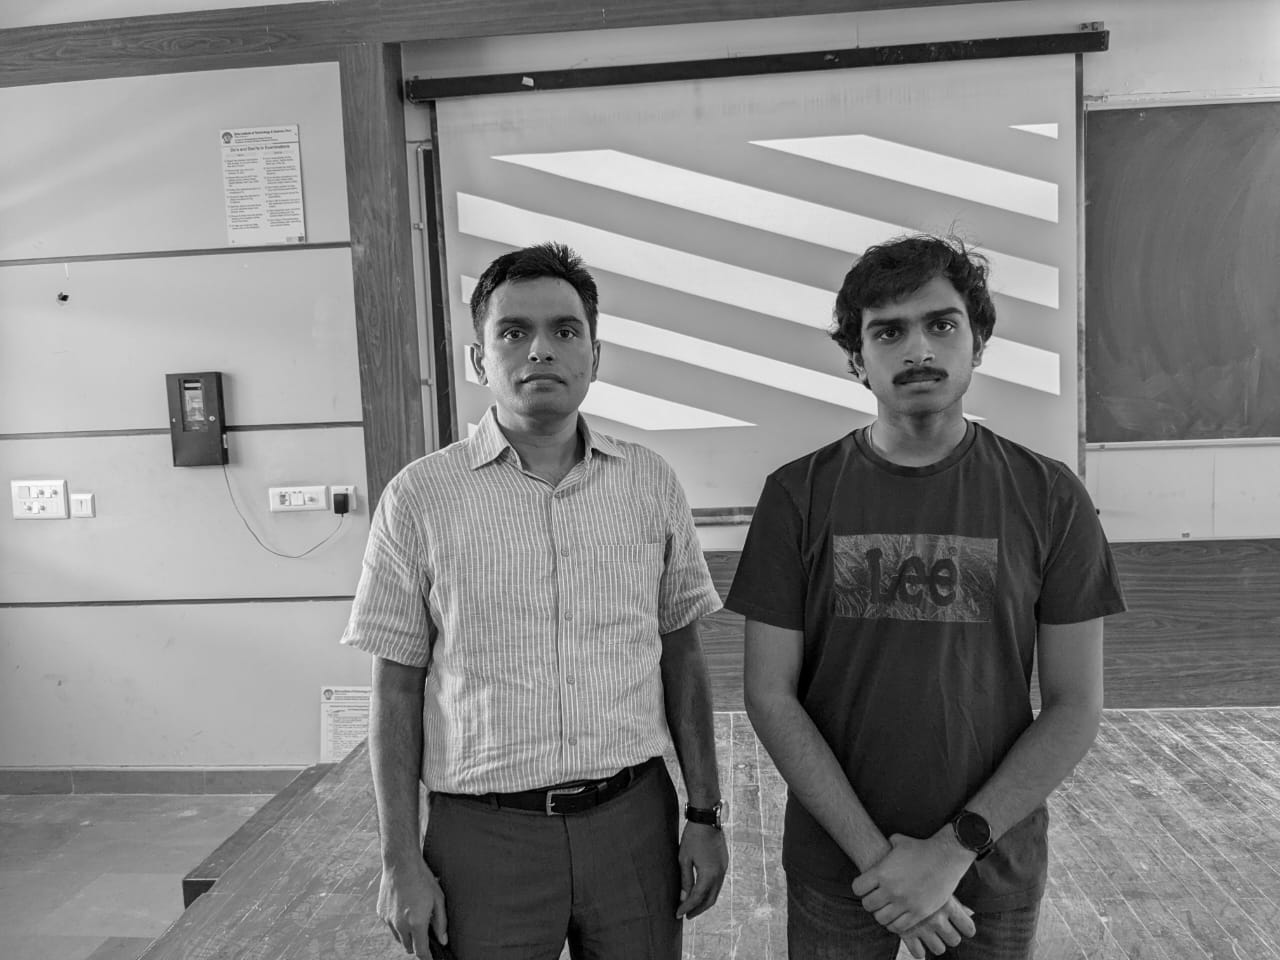
\includegraphics[width=\textwidth]{images/Image03_Original.png}
		\caption{Original}
	\end{subfigure}
	\hfill
	\begin{subfigure}[t]{0.23\textwidth}
		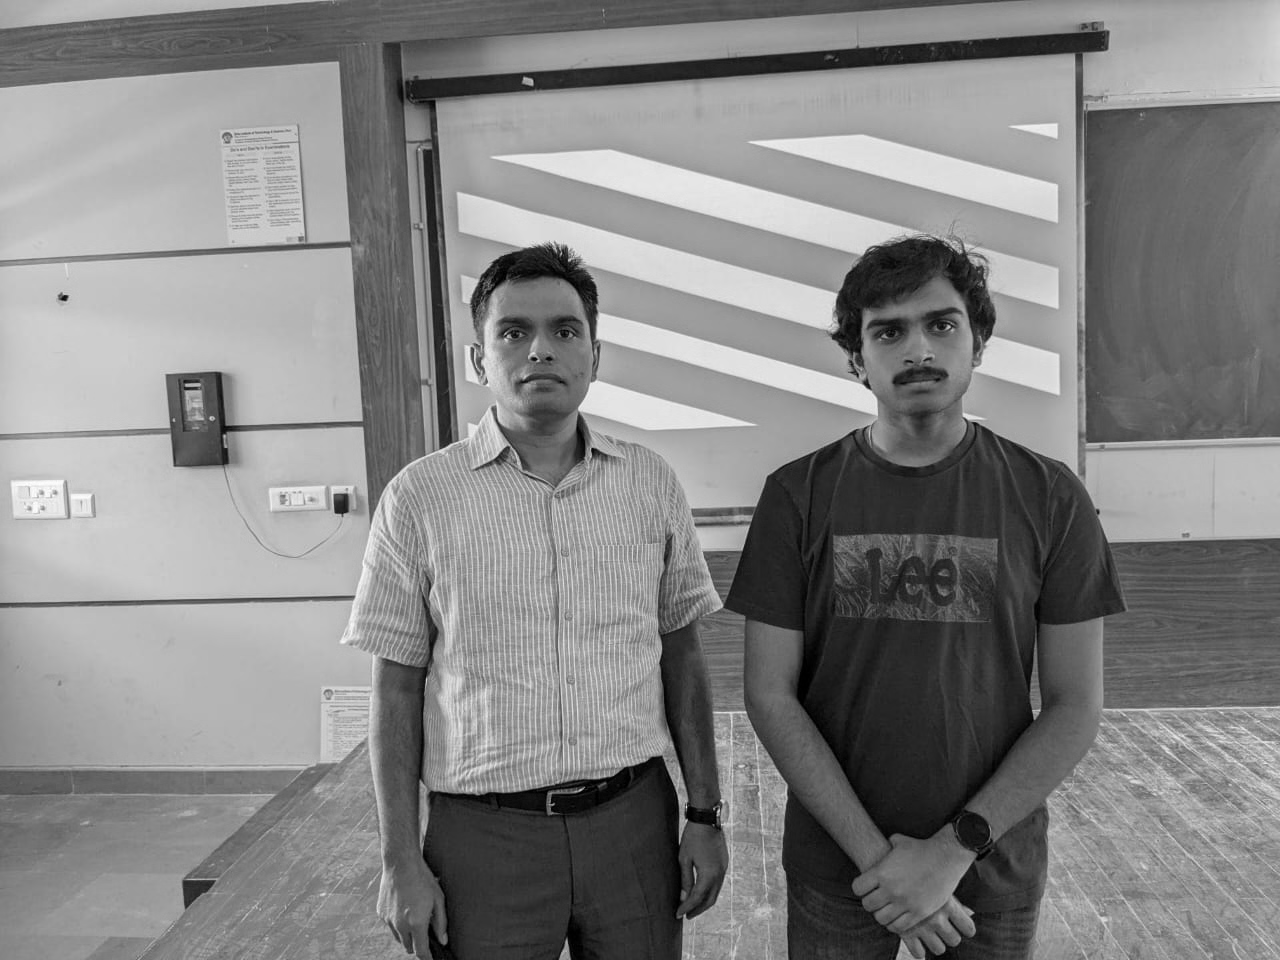
\includegraphics[width=\textwidth]{images/Image03_BTC.png}
		\caption{BTC}
	\end{subfigure}
	\hfill
	\begin{subfigure}[t]{0.23\textwidth}
		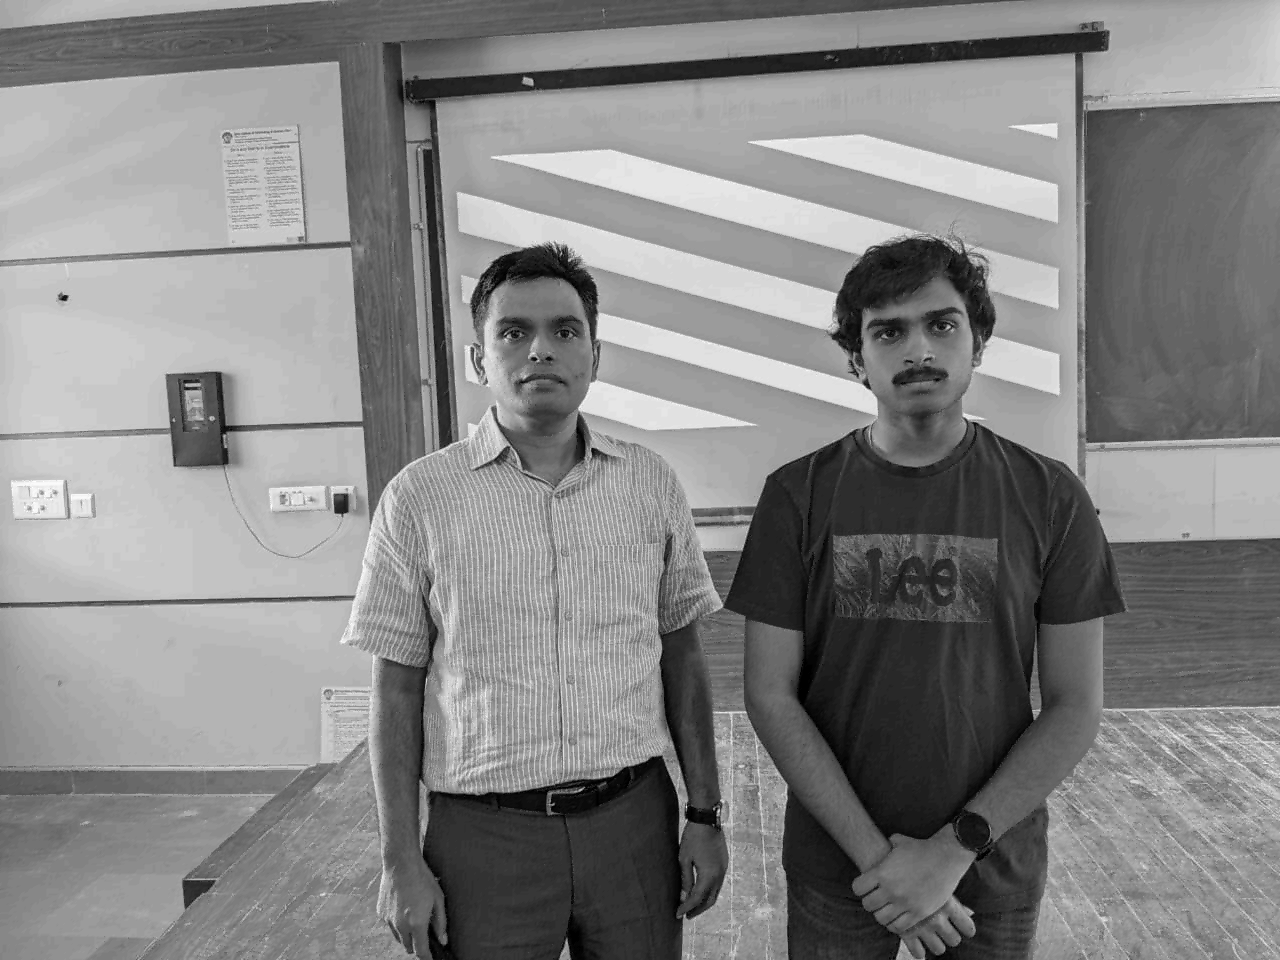
\includegraphics[width=\textwidth]{images/Image03_DPCM.png}
		\caption{DPCM}
	\end{subfigure}
	\hfill
	\begin{subfigure}[t]{0.23\textwidth}
		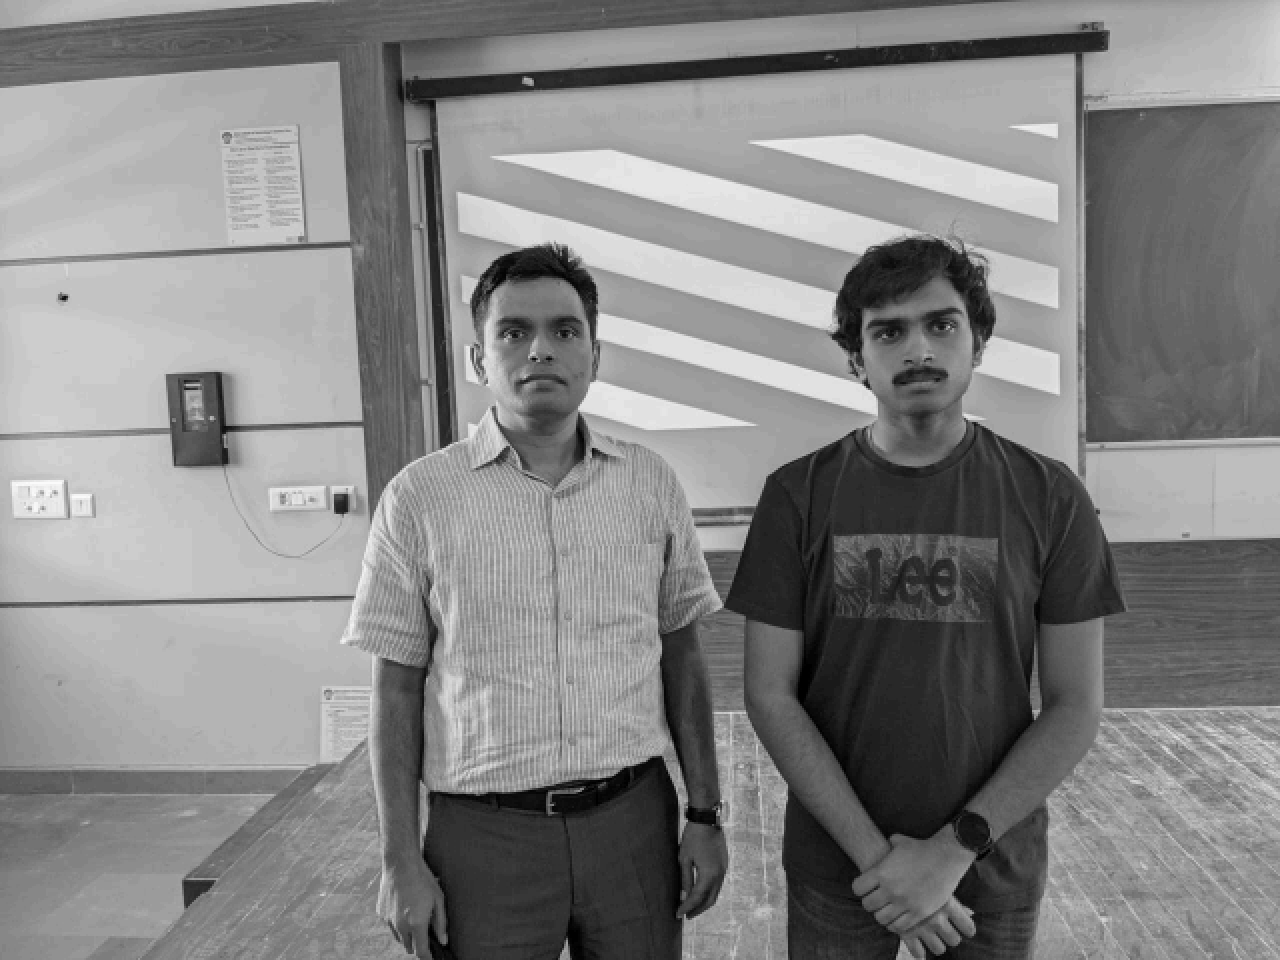
\includegraphics[width=\textwidth]{images/Image03_DWT.png}
		\caption{DWT}
	\end{subfigure}
	\caption{Image 2 Grayscale - Compression Comparison}
	\label{fig:img2-gray-comparison}
	
	\vspace{1.5cm}
	
	\begin{subfigure}[t]{0.23\textwidth}
		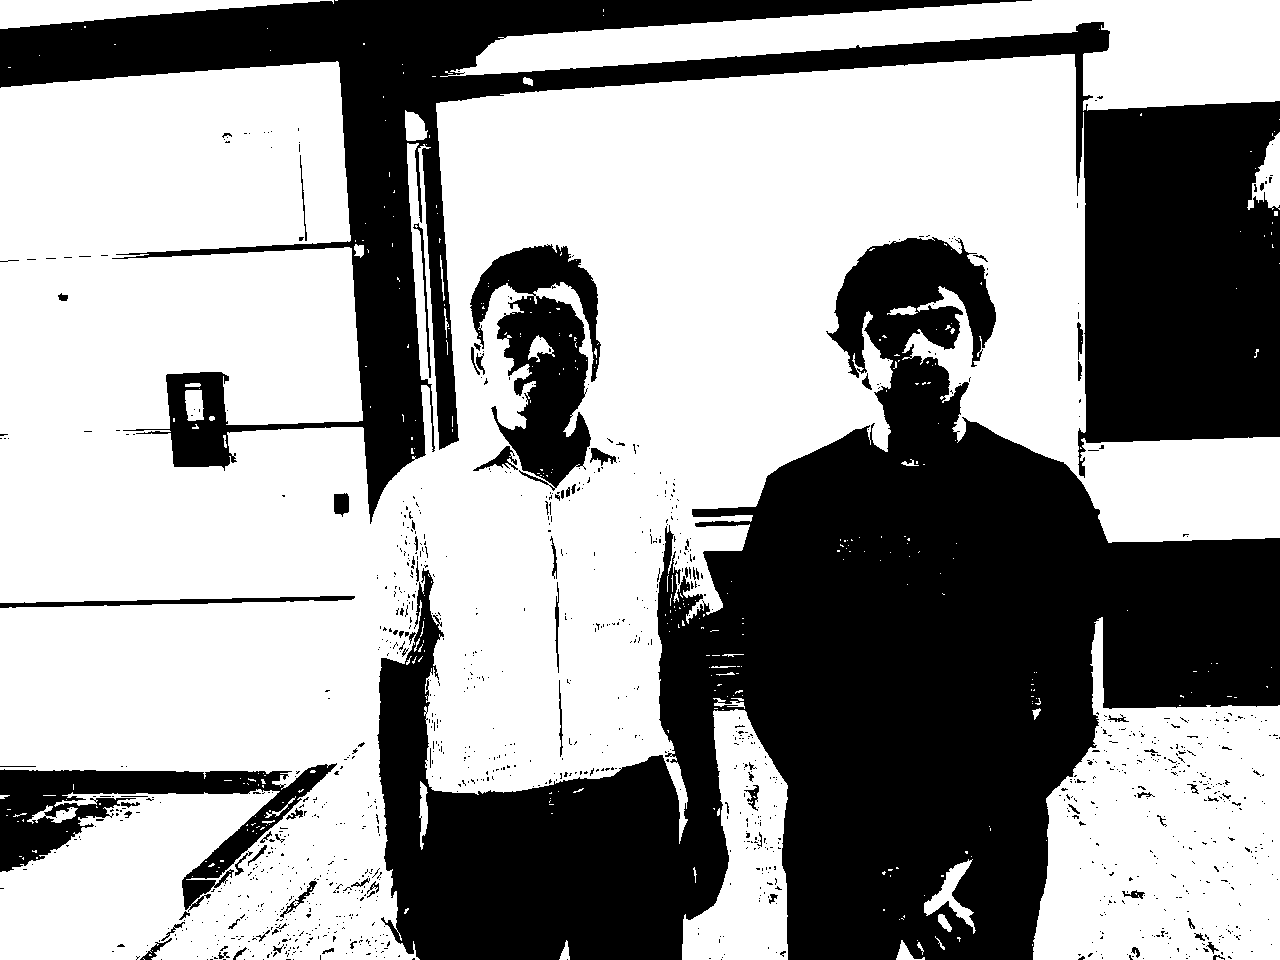
\includegraphics[width=\textwidth]{images/Image04_Original.png}
		\caption{Original}
	\end{subfigure}
	\hfill
	\begin{subfigure}[t]{0.23\textwidth}
		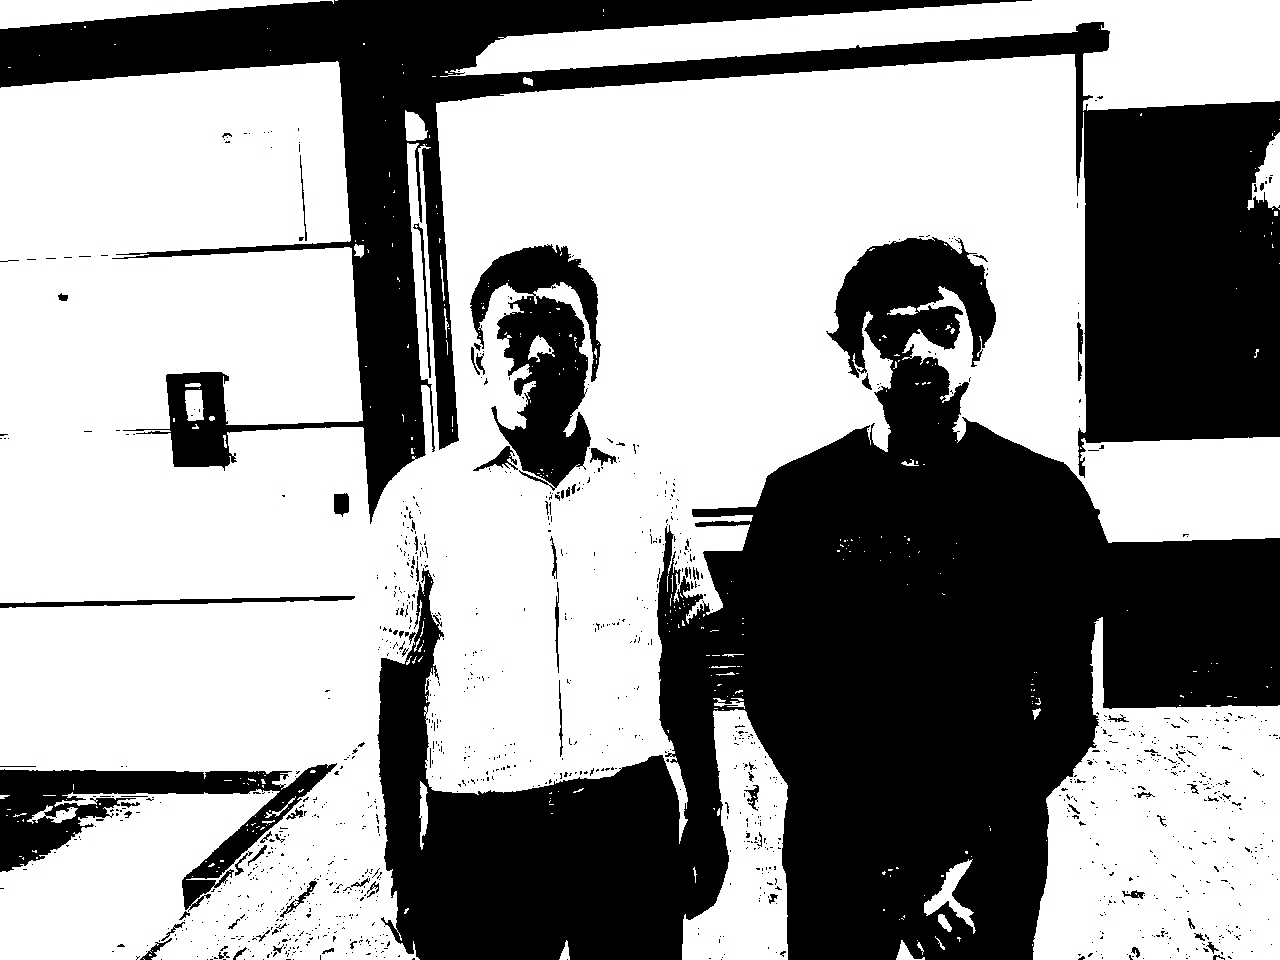
\includegraphics[width=\textwidth]{images/Image04_BTC.png}
		\caption{BTC}
	\end{subfigure}
	\hfill
	\begin{subfigure}[t]{0.23\textwidth}
		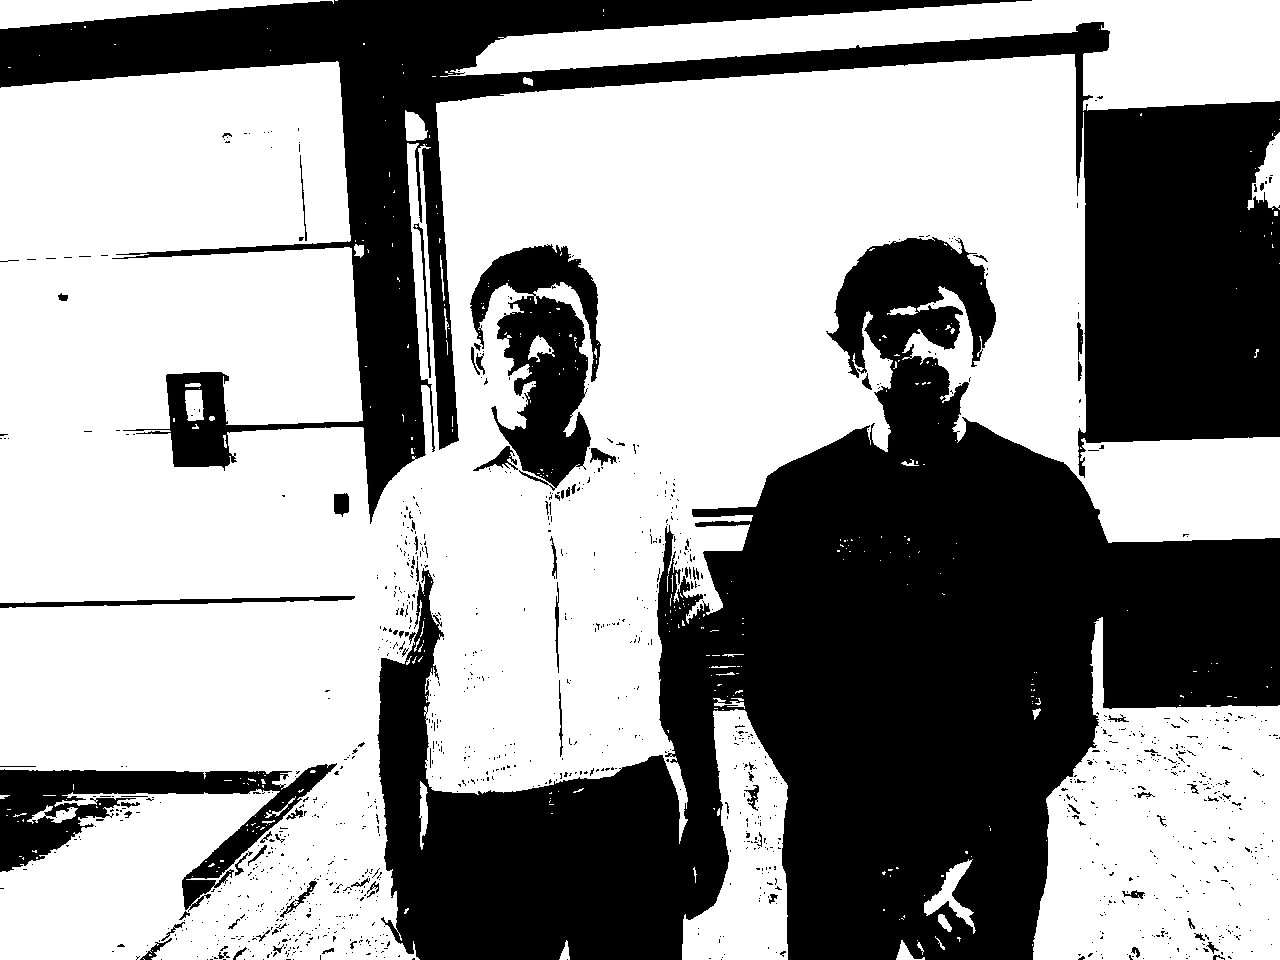
\includegraphics[width=\textwidth]{images/Image04_DPCM.png}
		\caption{DPCM}
	\end{subfigure}
	\hfill
	\begin{subfigure}[t]{0.23\textwidth}
		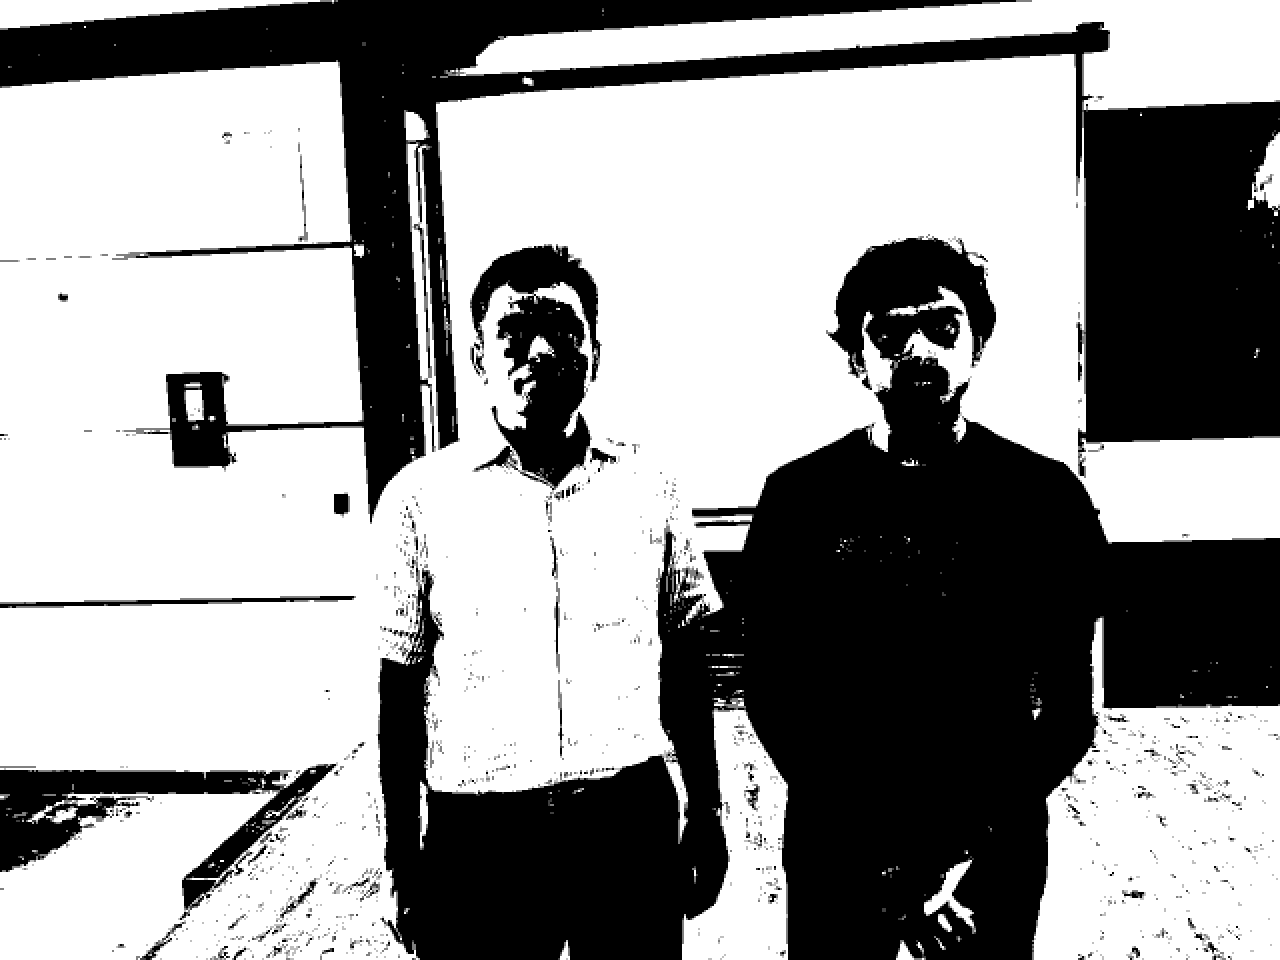
\includegraphics[width=\textwidth]{images/Image04_DWT.png}
		\caption{DWT}
	\end{subfigure}
	\caption{Image 2 Binary - Compression Comparison}
	\label{fig:img2-bin-comparison}
\end{figure}

\begin{figure}[htbp]
	\centering
	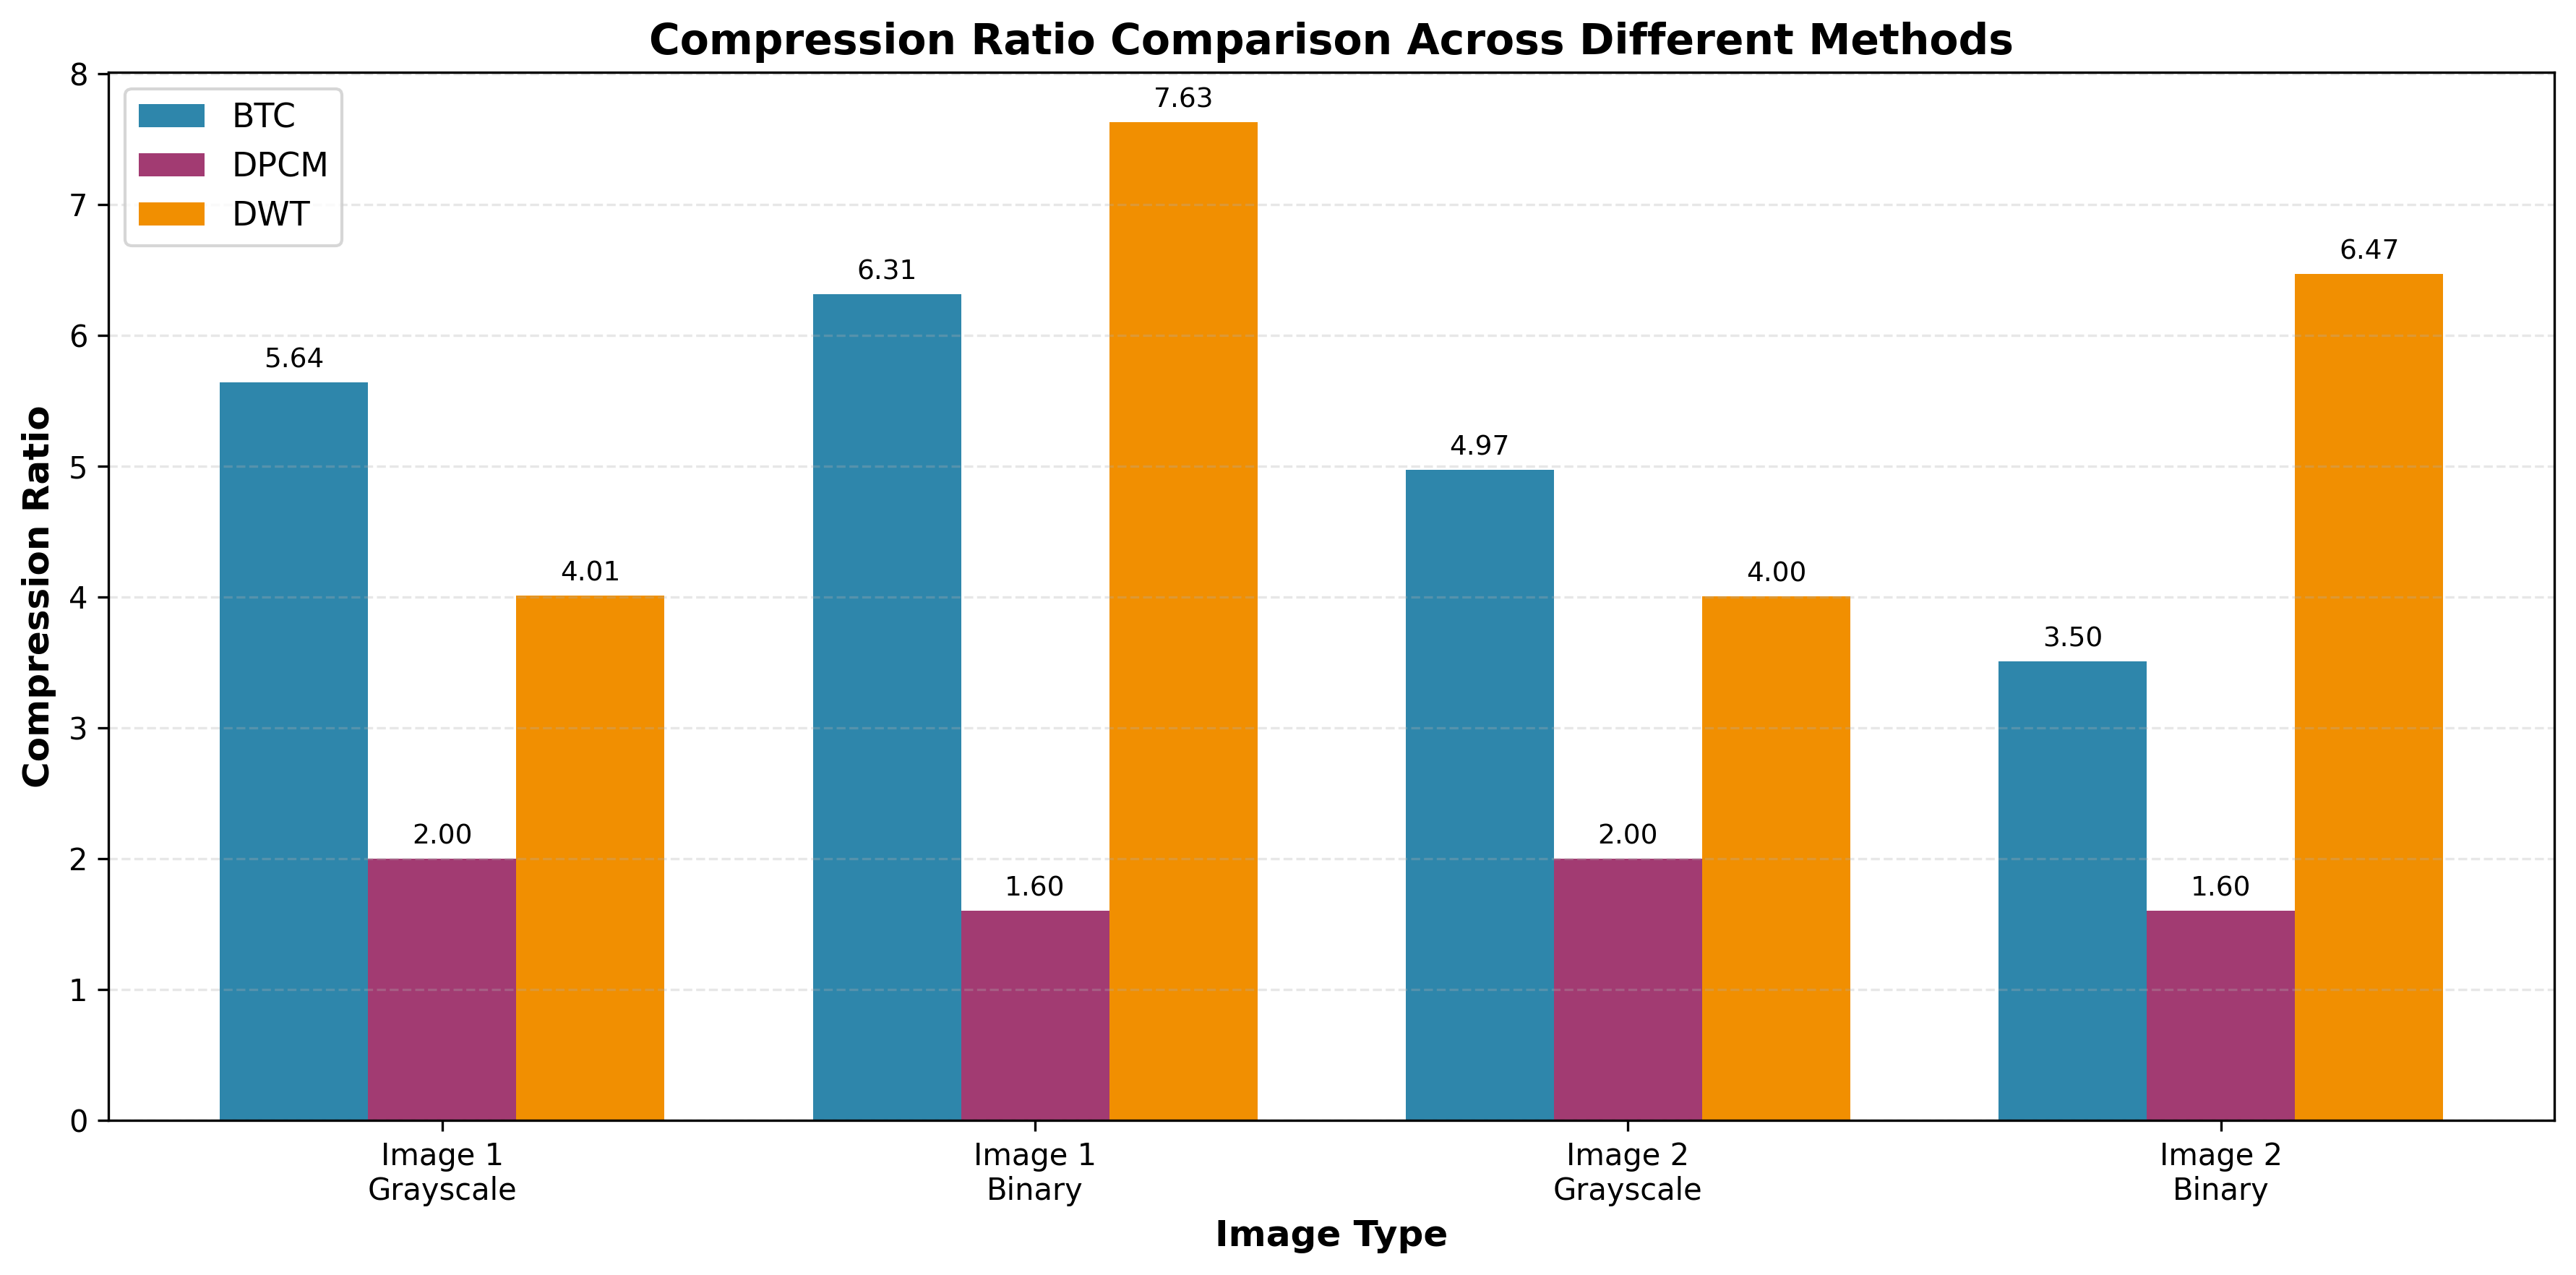
\includegraphics[width=0.85\textwidth]{images/compression-comparison-chart.png}
	\caption{Compression Ratio Comparison Across All Methods}
	\label{fig:compression-comparison}
\end{figure}

\subsection{Comparative Analysis}
\label{subsec:comparative-analysis}

\subsubsection{Binary Image Comparison}
For binary images (Images 2 and 4), the following observations were made:
\begin{itemize}
	\item \textbf{BTC} achieved good compression ratios (3.5--6.3) with excellent quality preservation (PSNR > 53 dB)
	\item \textbf{DPCM} provided consistent but conservative compression (CR $\approx$ 1.6) with high quality (PSNR > 53 dB)
	\item \textbf{Wavelet} achieved the highest compression ratios (6.5--7.6) but with significant quality degradation (PSNR < 24 dB)
\end{itemize}

The poor performance of wavelet coding on binary images is expected, as the averaging operation in the LL subband heavily smooths sharp edges, which are abundant in binary images. Binary images contain primarily high-frequency content (edges), which is discarded in the LL-only approach.

\subsubsection{Grayscale Image Comparison}
For grayscale images (Images 1 and 3), the results showed:
\begin{itemize}
	\item \textbf{BTC} delivered the best overall performance with compression ratios of 4.97--5.64 and excellent quality (PSNR > 46 dB)
	\item \textbf{DPCM} provided stable compression (CR = 2.0) with acceptable quality (PSNR > 36 dB)
	\item \textbf{Wavelet} achieved moderate compression (CR $\approx$ 4.0) with acceptable quality (PSNR > 32 dB)
\end{itemize}

Grayscale images typically contain more low-frequency content, which is better preserved by all three methods. BTC's DCT-based approach is particularly well-suited for natural images, as it can effectively separate and quantize frequency components.

\subsubsection{Binary vs Grayscale Comparison}
Key differences between binary and grayscale image compression:
\begin{itemize}
	\item Binary images generally achieved higher compression ratios with BTC and wavelet methods
	\item DPCM performed more conservatively on binary images (lower CR) but maintained higher quality
	\item The quality-compression trade-off is more severe for binary images with wavelet coding
	\item BTC showed more consistent quality across both image types
\end{itemize}

\subsection{Algorithm Selection Guidelines}
\label{subsec:algorithm-selection}
Based on the experimental results, the following guidelines are recommended:

\subsubsection{When to Use Block Transform Coding}
\textbf{Recommended for:}
\begin{itemize}
	\item Natural grayscale images requiring good compression with high quality
	\item Scenarios where PSNR > 45 dB is required
	\item Applications needing a balance between compression ratio (4--6) and visual quality
	\item JPEG-style compression for photographs and natural scenes
\end{itemize}

\textbf{Example:} Medical imaging, where diagnostic quality must be preserved while reducing storage requirements. A chest X-ray compressed with BTC at Q=5 maintains diagnostic features while achieving 5x compression.

\subsubsection{When to Use Predictive Coding}
\textbf{Recommended for:}
\begin{itemize}
	\item Applications where quality is paramount over compression ratio
	\item Images with smooth gradients and high spatial correlation
	\item Real-time compression where computational simplicity is valued
	\item Lossless or near-lossless compression requirements
\end{itemize}

\textbf{Example:} Video conferencing systems, where consistent frame quality is more important than high compression. DPCM ensures predictable quality (PSNR > 35 dB) with low computational overhead.

\subsubsection{When to Use Wavelet Coding}
\textbf{Recommended for:}
\begin{itemize}
	\item Applications requiring progressive transmission
	\item Scenarios where very high compression ratios are needed and quality can be sacrificed
	\item Multi-resolution analysis requirements
	\item When additional high-frequency subbands are retained (not just LL)
\end{itemize}

\textbf{Example:} Satellite imagery thumbnails or preview generation, where the LL subband provides a quick overview. The high compression ratio (7x) enables fast transmission, and full quality can be loaded on demand.

\textbf{Note:} The poor performance on binary images in this study is due to the LL-only implementation. A full wavelet implementation retaining all subbands would perform significantly better.

\subsection{Summary of Image Compression Results}
\label{subsec:image-compression-summary}
Table \ref{tab:image-compression-summary} provides a comprehensive summary of all compression results.

\begin{table}[h!]
	\centering
	\small
	\begin{adjustbox}{max width=\textwidth}
	\begin{tabular}{lcccccc}
		\toprule
		\textbf{Image} & \textbf{BTC CR} & \textbf{BTC PSNR} & \textbf{DPCM CR} & \textbf{DPCM PSNR} & \textbf{DWT CR} & \textbf{DWT PSNR} \\
		\midrule
		Image 1 Gray & 5.640 & 46.86 & 2.000 & 38.51 & 4.008 & 35.67 \\
		Image 1 Binary & 6.311 & 56.53 & 1.600 & 55.79 & 7.627 & 23.52 \\
		Image 2 Gray & 4.970 & 48.38 & 2.000 & 36.19 & 4.002 & 32.12 \\
		Image 2 Binary & 3.504 & 53.12 & 1.600 & 53.86 & 6.469 & 21.47 \\
		\midrule
		\textbf{Average} & \textbf{5.106} & \textbf{51.22} & \textbf{1.800} & \textbf{46.09} & \textbf{5.527} & \textbf{28.20} \\
		\bottomrule
	\end{tabular}
	\end{adjustbox}
	\caption{Comprehensive Summary of Image Compression Results}
	\label{tab:image-compression-summary}
\end{table}

\section{Conclusion}
\label{sec:conclusion}
This assignment successfully implemented and analyzed multiple compression algorithms for both text and image data.

For text compression, LZW demonstrated superior performance on the test strings, achieving compression ratios of 1.217 (short string) and 2.014 (long string). The analysis revealed that compression effectiveness increases significantly with input length, as dictionary-based methods can better exploit redundancy in longer sequences. Window size analysis for LZ77 showed that optimal parameters depend on input characteristics, with both excessively small and large windows degrading performance.

For image compression, Block Transform Coding emerged as the best overall method for quality-sensitive applications, achieving compression ratios of 4--6 while maintaining PSNR values above 46 dB for grayscale images. DPCM provided the most consistent and reliable compression across different image types, making it suitable for applications prioritizing stability. Wavelet coding showed promise for high-compression scenarios but requires retention of additional subbands beyond LL-only for acceptable quality on binary images.

The key takeaway is that compression algorithm selection must consider the specific characteristics of the input data and application requirements. No single algorithm performs optimally across all scenarios, emphasizing the importance of understanding the fundamental trade-offs between compression ratio, computational complexity, and reconstruction quality.

\newpage
\appendix
\section{Code Listings}
\label{appendix:code-listings}
\subsection{LZ77 Compression Code}
\label{subappendix:lz77-code}
\begin{lstlisting}[language=Matlab, caption={LZ77 Compression Implementation}, label={lst:lz77-code}]
function tokens = lz77_compress(s, searchSize, lookaheadSize)
s = char(s);
n = length(s);
pos = 1;
tokens = {};
idx = 0;

while pos <= n
    windowStart = max(1, pos - searchSize);
    window = s(windowStart:pos-1);
    bestLen = 0;
    bestOffset = 0;
    laMax = min(lookaheadSize, n - pos + 1);

    for L = laMax:-1:1
        substr = s(pos:pos+L-1);
        matchPos = strfind(window, substr);
        if ~isempty(matchPos)
            last = matchPos(end);
            matchStart = windowStart + last - 1;
            bestOffset = pos - matchStart;
            bestLen = L;
            break
        end
    end

    idx = idx + 1;
    if bestLen == 0
        tokens{idx} = struct('offset',0,'len',0,'next',s(pos));
        pos = pos + 1;
    else
        if pos+bestLen <= n
            nextChar = s(pos+bestLen);
            pos = pos + bestLen + 1;
        else
            nextChar = '';
            pos = pos + bestLen;
        end
        tokens{idx} = struct('offset',bestOffset,'len',bestLen,'next',nextChar);
    end
end
end
\end{lstlisting}

\subsection{LZ78 Compression Code}
\label{subappendix:lz78-code}
\begin{lstlisting}[language=Matlab, caption={LZ78 Compression Implementation}, label={lst:lz78-code}]
function [pairs, dict, total_bits] = lz78_pairs_only(s)

s = char(s);
dict = {""};
pairs = {};
n = length(s);
i = 1;

while i <= n
    prefixIdx = 0;
    j = i;

    while j <= n
        cand = s(i:j);
        found = find(strcmp(dict,cand),1);
        if ~isempty(found)
            prefixIdx = found - 1;
            j = j + 1;
        else
            break
        end
    end

    if j <= n
        nextChar = s(j);
        newEntry = s(i:j);
        dict{end+1} = newEntry;
        pairs{end+1} = struct('index',prefixIdx,'next',nextChar);
        i = j + 1;
    else
        newEntry = s(i:j-1);
        dict{end+1} = newEntry;
        pairs{end+1} = struct('index',prefixIdx,'next','');
        break
    end
end

max_index = 0;

for k = 1:length(pairs)
    max_index = max(max_index, pairs{k}.index);
end

idx_bits = max(1, ceil(log2(max_index + 1)));   % at least 1 bit
total_bits = 0;
for k = 1:length(pairs)
    total_bits = total_bits + idx_bits;      % index bits
    if ~isempty(pairs{k}.next)
        total_bits = total_bits + 8;  % literal bit
    end
end

end
\end{lstlisting}

\subsection{LZ77 Decompression Code}
\label{subappendix:lz77-decompress-code}
\begin{lstlisting}[language=Matlab, caption={LZ77 Decompression Implementation}, label={lst:lz77-decompress-code}]
function out = lz77_decompress(tokens)
out = '';
for i = 1:numel(tokens)
    t = tokens{i};
    if t.offset == 0 && t.len == 0
        % No match found, append the literal character
        out = [out t.next];
    else
        % Match found, copy from earlier in the output
        startIdx = numel(out) - t.offset + 1;
        
        % Safety check to ensure valid offset
        if startIdx < 1
            error('Invalid offset during LZ77 decompression.');
        end
        
        % Extract the matched sequence
        seq = out(startIdx : startIdx + t.len - 1);
        out = [out seq];
        
        % Append the next character if it exists
        if ~isempty(t.next)
            out = [out t.next];
        end
    end
end
end
\end{lstlisting}

\subsection{Block Transform Coding Implementation}
\label{subappendix:btc-code}
\begin{lstlisting}[language=Matlab, caption={Block Transform Coding Implementation}, label={lst:btc-code}]
function [bits, rec] = block_transform_coding(img, blk, Q)
% BLOCK_TRANSFORM_CODING  Block DCT + quantization + entropy bit estimate
%   [bits, rec] = block_transform_coding(img, blk, Q)
%   - img: double image (0..255)
%   - blk: block size (e.g. 16)
%   - Q:   scalar quantizer step
%
% The function returns:
%  - bits : estimated compressed bit count (entropy-coded estimate)
%  - rec  : reconstructed image after dequantize + idct

[H,W] = size(img);

% Pad to multiple of block size
padH = ceil(H / blk) * blk;
padW = ceil(W / blk) * blk;
padded = zeros(padH, padW);
padded(1:H,1:W) = img;

rec = zeros(padH, padW);

% Collect quantized coefficients (in zigzag order) from all blocks
all_coeffs = [];

for r = 1:blk:padH
    for c = 1:blk:padW
        block = padded(r:r+blk-1, c:c+blk-1);
        C = dct2(block);

        % Uniform scalar quantization
        Cq = round(C / Q);

        % Zig-zag scan the block to get a 1D vector (DC first)
        v = zigzag_scan(Cq);
        all_coeffs = [all_coeffs; v(:)];

        % Reconstruct block into rec buffer
        rec(r:r+blk-1, c:c+blk-1) = idct2(Cq * Q);
    end
end

% Crop reconstructed image to original size
rec = rec(1:H,1:W);
rec(rec<0) = 0;
rec(rec>255) = 255;

% Entropy bit estimate
coeffs = all_coeffs(:);

if all(coeffs == 0)
    bits_entropy = 1;   % trivial case
else
    % Compute occurrences
    [sym_vals, ~, idx_map] = unique(coeffs);
    counts = accumarray(idx_map, 1);
    total = sum(counts);

    p = counts ./ total;               % empirical probabilities
    bits_per_symbol = -log2(p);        % ideal bits per symbol
    bits_entropy = sum(counts .* bits_per_symbol);  % total entropy bits
end

% Add small header overhead
header_bits = 64;

bits = ceil(bits_entropy + header_bits);

end

function vec = zigzag_scan(A)
% Produces a zig-zag scan (DC first) of a square block A
[blk1, blk2] = size(A);
if blk1 ~= blk2
    error('zigzag_scan expects square blocks');
end
N = blk1;

vec = zeros(N*N,1);
k = 1;
for s = 0:(2*(N-1))
    if mod(s,2) == 0
        % even sum (go up)
        i_start = max(0, s-(N-1));
        i_end   = min(N-1, s);
        for i = i_start:i_end
            j = s - i;
            vec(k) = A(i+1, j+1);
            k = k + 1;
        end
    else
        % odd sum (go down)
        j_start = max(0, s-(N-1));
        j_end   = min(N-1, s);
        for j = j_start:j_end
            i = s - j;
            vec(k) = A(i+1, j+1);
            k = k + 1;
        end
    end
end
end
\end{lstlisting}

\subsection{Predictive Coding (DPCM) Implementation}
\label{subappendix:dpcm-code}
\begin{lstlisting}[language=Matlab, caption={Predictive Coding (DPCM) Implementation}, label={lst:dpcm-code}]
function [bits, rec] = predictive_coding(img, Q)

img = double(img);
[H, W] = size(img);

% Step 1: Quantize image
img_q = round(img / Q);

% Step 2: Predictor matrix
pred = zeros(H, W);

for i = 1:H
    for j = 1:W
        
        if i == 1 && j == 1
            pred(i,j) = 0;                          % Rule 1: top-left
        
        elseif j == 1
            pred(i,j) = img_q(i-1, j);              % Rule 2: left column
        
        elseif i == 1
            pred(i,j) = img_q(i, j-1);              % Rule 3: top row
        
        else
            % Rule 4: average of top and left
            pred(i,j) = (img_q(i-1, j) + img_q(i, j-1)) / 2;
        end
        
    end
end

% Step 3: Compute error matrix
err = img_q - pred;

% Step 4: Quantize error
err_q = round(err / Q);

% Step 5: Bit estimate
maxErr = max(abs(err_q(:)));

if maxErr == 0
    bits_per_pixel = 1;   % minimal cost case
else
    bits_per_pixel = ceil(log2(2 * maxErr + 1));
end

bits = bits_per_pixel * H * W;

% Step 6: Reconstruct image
rec = pred + err_q * Q;

% Restore valid grayscale range
rec = rec * Q;
rec(rec < 0) = 0;
rec(rec > 255) = 255;

end
\end{lstlisting}

\subsection{Wavelet Coding Implementation}
\label{subappendix:dwt-code}
\begin{lstlisting}[language=Matlab, caption={Wavelet Coding (LL-only) Implementation}, label={lst:dwt-code}]
function [bits, rec] = wavelet_LL_only_quantized(img, Q)

img = double(img);
[H0,W0] = size(img);

% Fix odd sizes by padding
if mod(H0,2)==1, img(end+1,:) = img(end,:); end
if mod(W0,2)==1, img(:,end+1) = img(:,end); end
[H,W] = size(img);

% Quantize input
img_q = round(img / Q) * Q;

% 2D averaging-based wavelet transform
% Row-wise averaging
row_low = (img_q(:,1:2:end) + img_q(:,2:2:end)) / 2;

% Column-wise averaging to get LL subband
LL = (row_low(1:2:end,:) + row_low(2:2:end,:)) / 2;

% Bit model for LL coefficients
nz = LL(LL~=0);
if isempty(nz)
    bits = 32;   % header only
else
    maxAbs = max(abs(nz));
    bits_per_coeff = ceil(log2(maxAbs+1));
    bits = numel(nz) * bits_per_coeff + 32;  % include small header
end

% Reconstruction by upsampling
rec_low = repelem(LL,2,1);   % double rows
rec_full = repelem(rec_low,1,2); % double cols

% Crop to original size
rec = rec_full(1:H0, 1:W0);
rec(rec<0)=0; 
rec(rec>255)=255;

end
\end{lstlisting}

\end{document}
